\section{Casi d'uso}

\subsection{Scopo}
Questa sezione descrive nel dettaglio i Casi d’Uso individuati dal gruppo durante l'analisi.

\subsection{Attori}
Il prodotto prevede due attori:
\begin{itemize}
  \item Utente: un utente generico che ha accesso alle funzionalità richieste per la generazione di un \glossario{prompt} utilizzando i dizionari dati precaricati;
  \item Tecnico: un utente che ha completato con successo l'autenticazione ed è registrato come Tecnico, ha accesso a tutte le funzionalità dell'utente generico e in aggiunta può gestire i dizionari dati ed accedere a funzionalità di testing e debug.
\end{itemize}

\subsection{Gestione degli errori}
Alcuni dei casi d'uso gestiscono situazioni di errore, questo permette ai programmatori di gestire eventuali situazioni eccezionali, in modo che vengano intercettate e non portino ad un malfunzionamento del sistema, ma anzi gestite e notificate quando questo è utile.

\subsection{Elenco dei \glossario{casi d'uso}}

\subsubsection{UC1 - Autenticazione}\label{UC1}

\begin{figure}[H]
  \centering
  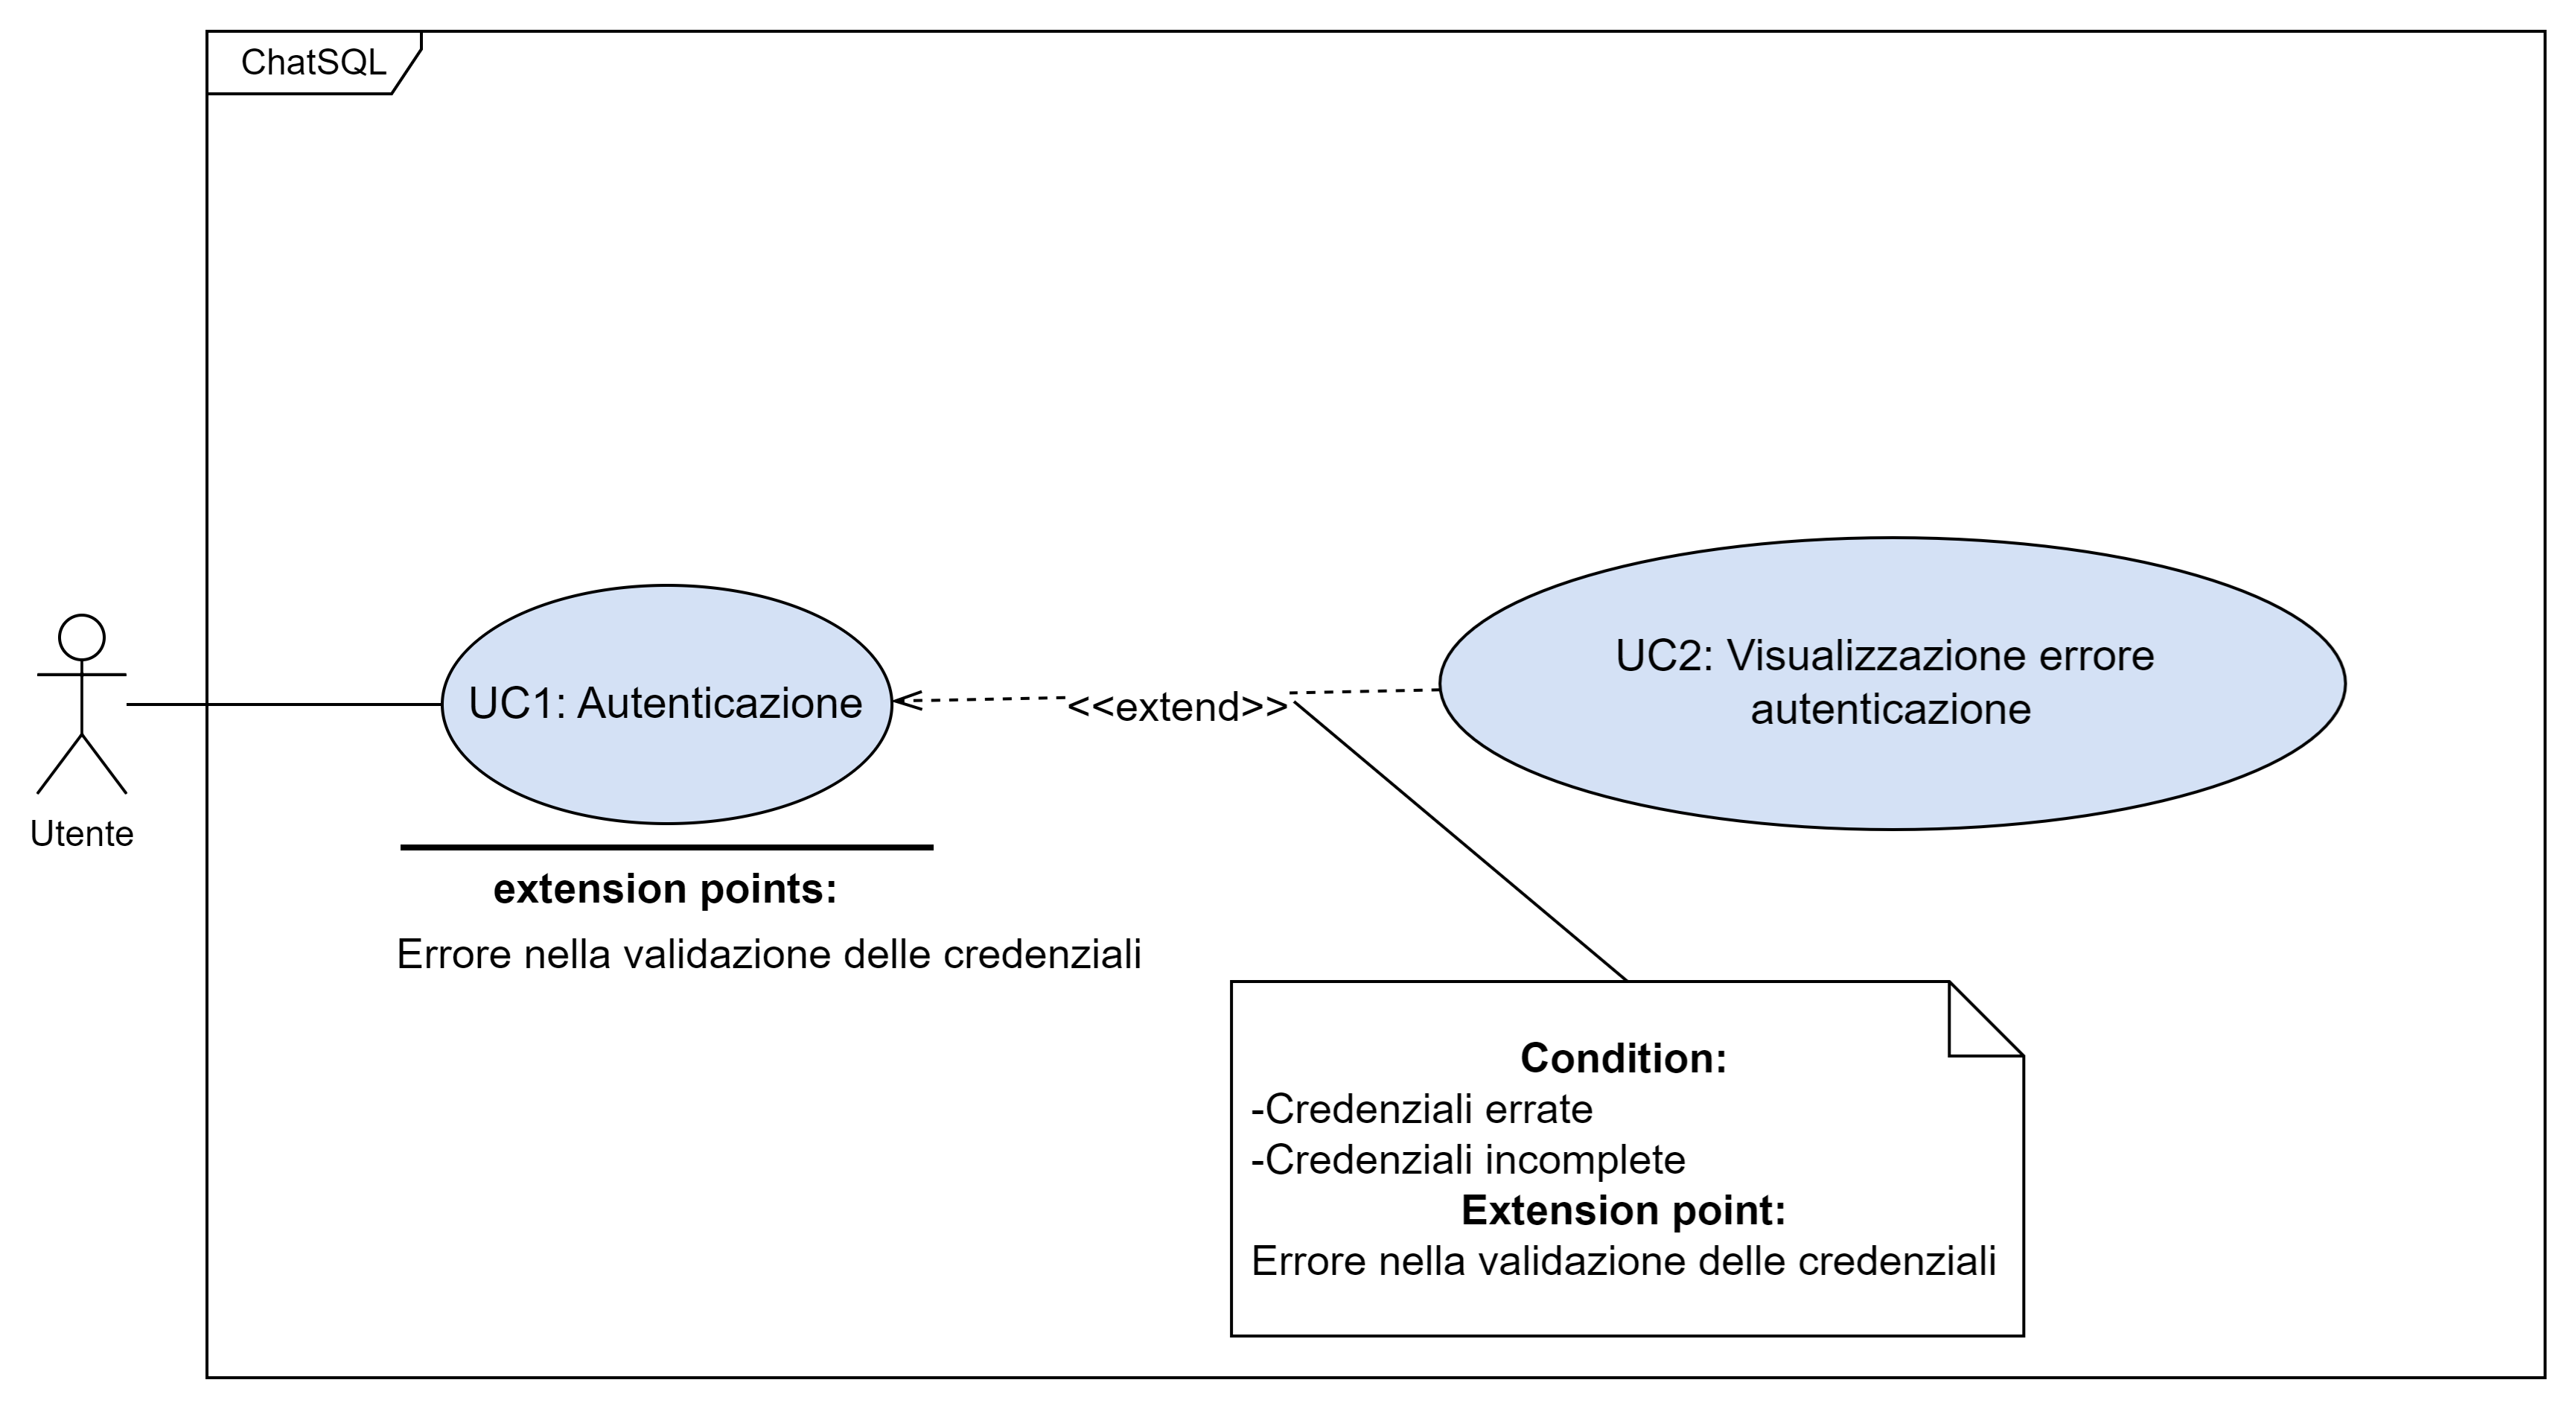
\includegraphics[width=0.95\textwidth]{assets/uc1.png}
  \caption{UC1}
\end{figure}

\paragraph*{Descrizione}
L'autenticazione corrisponde al processo di login, tramite il quale il Tecnico può ampliare le funzionalità disponibili.

\paragraph*{Attori principali}
Tecnico

\paragraph*{Precondizioni}
\begin{itemize}
  \item Il sistema è attivo e funzionante;
  \item Il Tecnico è stato registrato presso il sistema;
  \item Il Tecnico non è autenticato nella sessione corrente.
\end{itemize}

\paragraph*{Postcondizioni}
\begin{itemize}
  \item La procedura di autenticazione si è conclusa con successo;
  \item Il Tecnico visualizza le funzionalità aggiuntive nell'interfaccia.  
\end{itemize}

\paragraph*{Trigger}
Il Tecnico desidera accedere all'area di amministrazione.

\paragraph*{Scenario principale}
\begin{itemize}
  \item Il Tecnico seleziona l'opzione "Login";
  \item Il Tecnico inserisce le proprie credenziali;
  \item Il Tecnico effettua l'accesso;
  \item Il sistema mostra la schermata aggiornata con le funzionalità disponibili.
\end{itemize}

\paragraph*{Scenario alternativo}
\begin{enumerate}
  \item Il sistema riscontra un errore durante la validazione delle credenziali (\hyperref[UC2]{UC2});
  \item Viene visualizzato un messaggio con i dettagli dell'errore.
\end{enumerate}

\paragraph*{Estensioni}
\begin{itemize}
  \item Visualizzazione errore autenticazione (\hyperref[UC2]{UC2}).
  \begin{itemize}
    \item Extension point: Errore nella validazione delle credenziali;
    \item Condition: Credenziali errate, credenziali incomplete.
  \end{itemize}
\end{itemize}

% al posto dell'inclusione forse basta il sottocaso d'uso
\paragraph*{Sottocasi d'uso:}
\begin{itemize}
  \item UC1.1: Inserimento username;
  \item UC1.2: Inserimento password.
\end{itemize}

\begin{figure}[H]
  \centering
  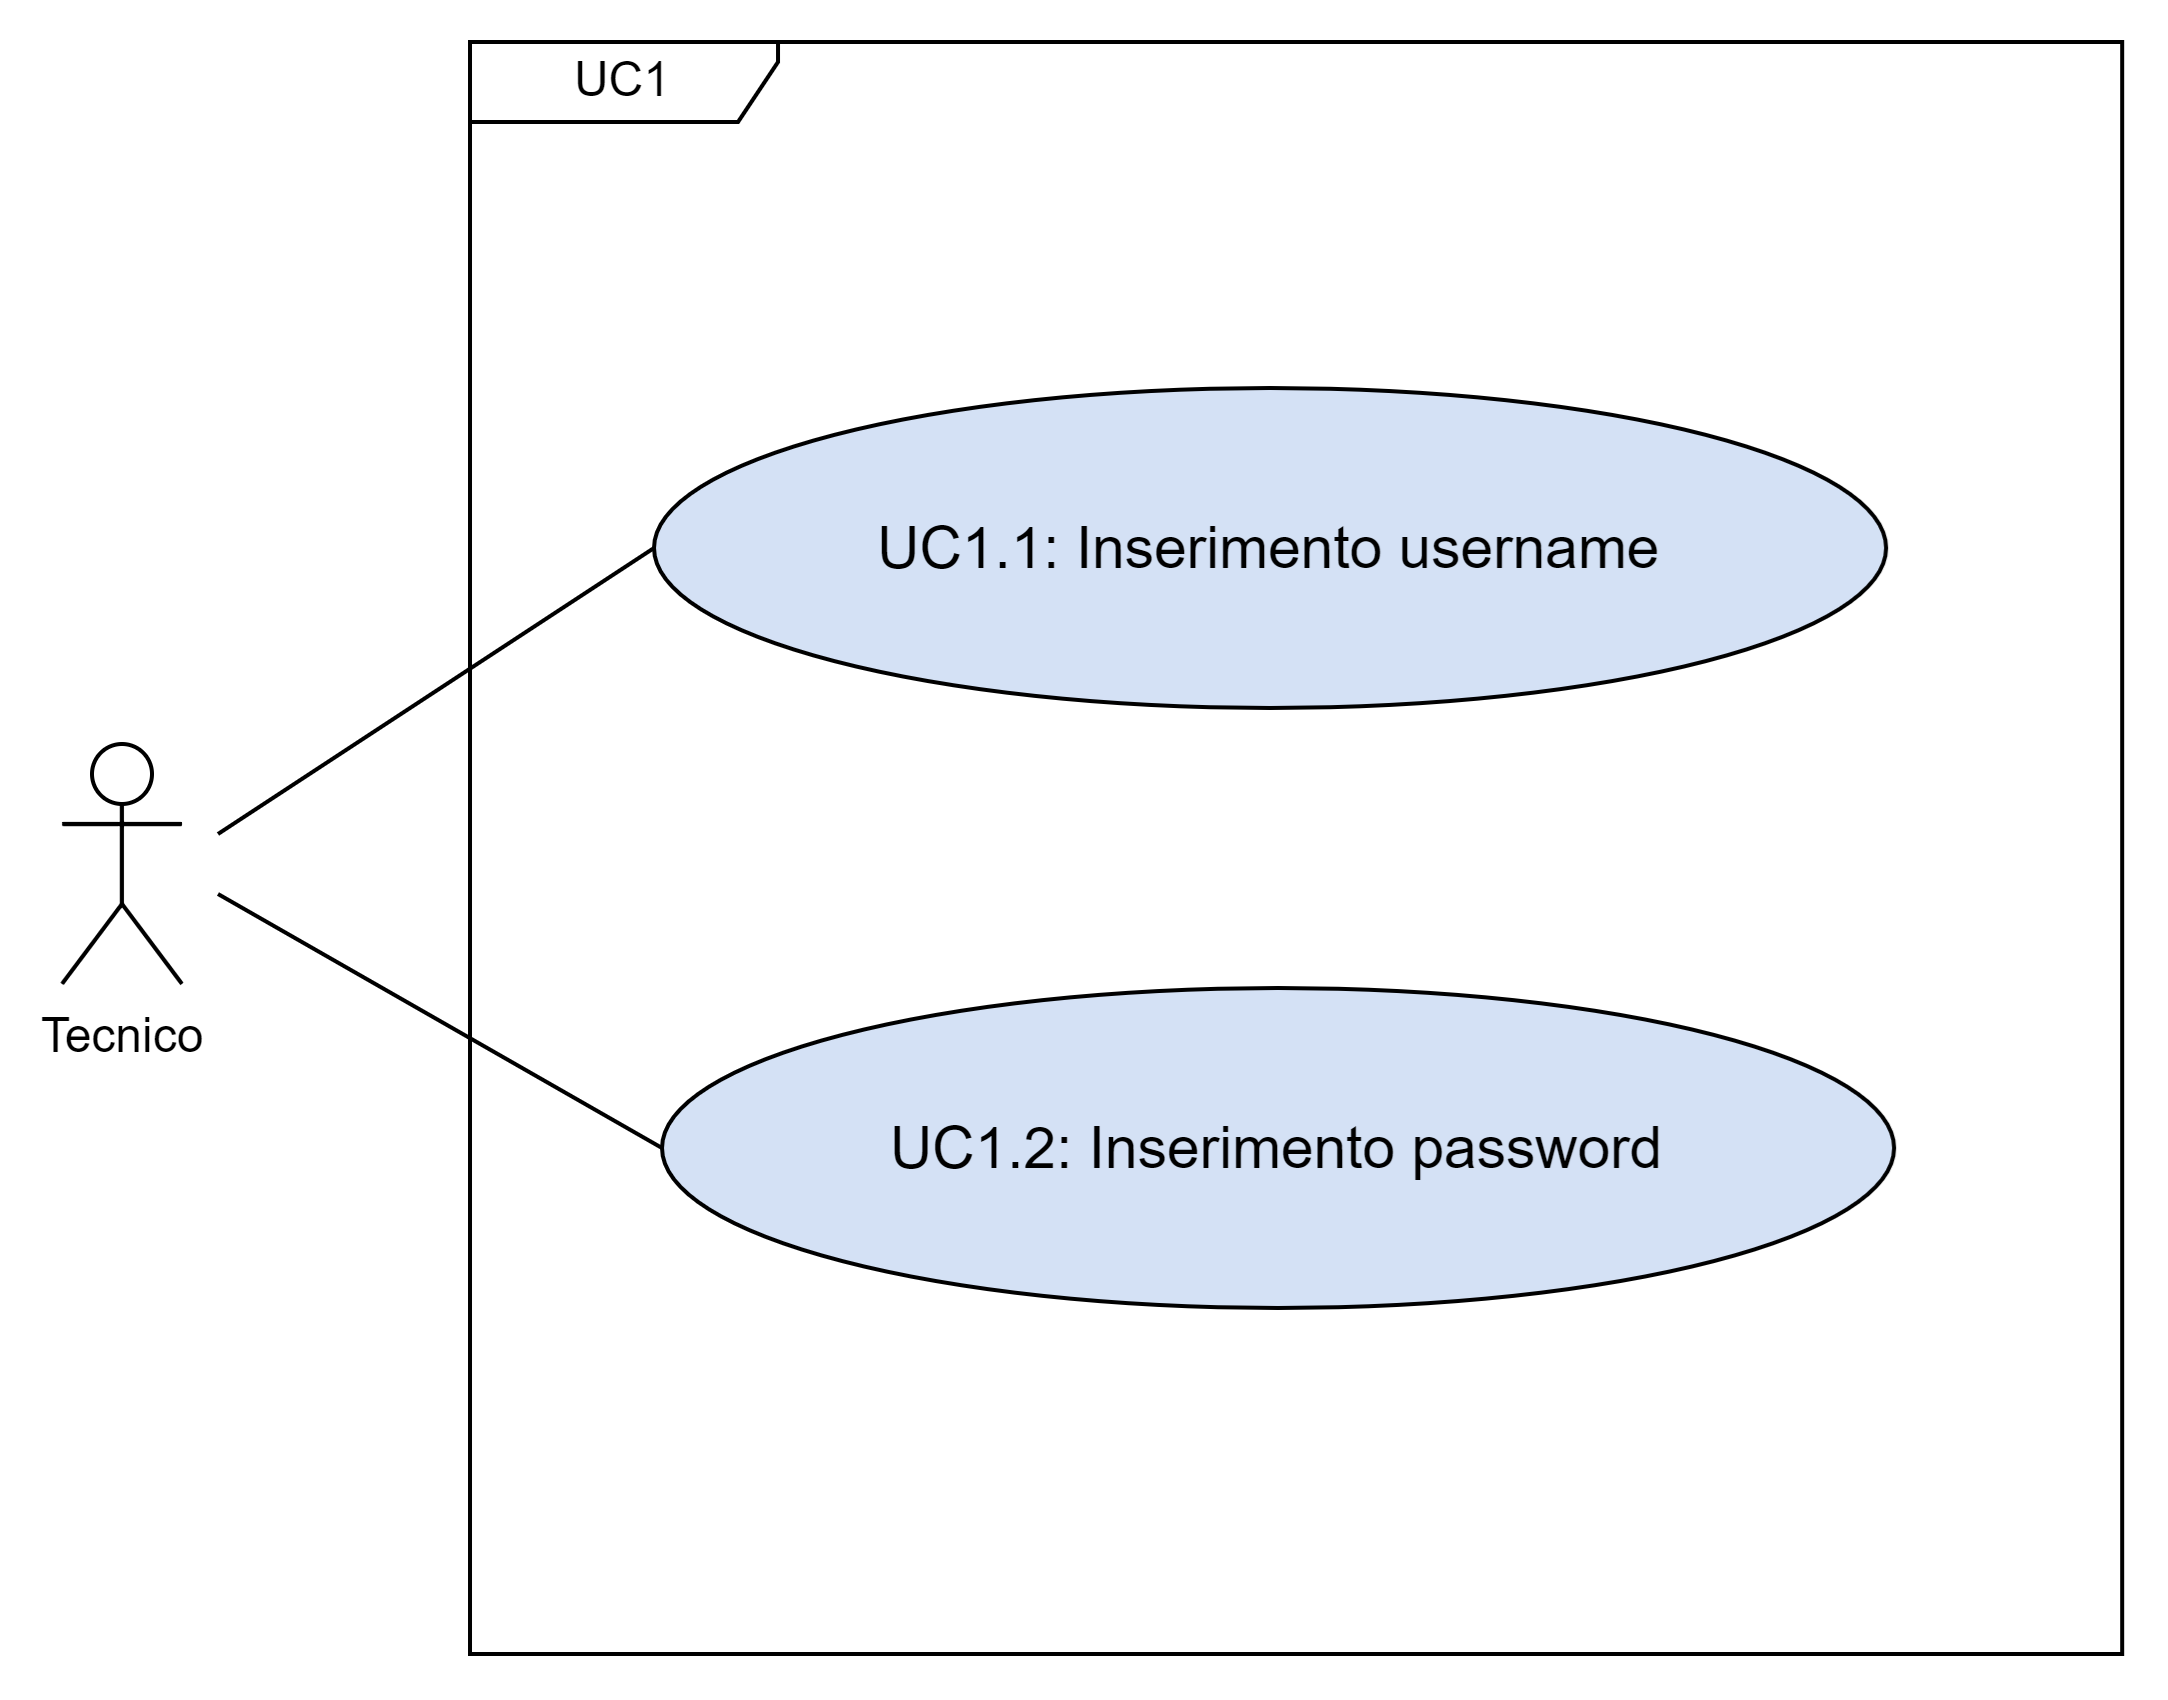
\includegraphics[width=0.90\textwidth]{assets/uc1_1.png}
  \caption{UC1 - Sottocasi d'uso}
\end{figure}

%%%%%%%%%%%%%%%%%%%%%%%%%%%%%%%%%%%%%%%%%%%%%%%%%%%%%%%%%%%%%%%%%%%%%%%%%%%%%%

\subsubsection{UC1.1 - Inserimento username}\label{UC1point1}

\paragraph*{Descrizione}
La procedura di "inserimento username" corrisponde all'immissione del nome utente nella sezione apposita di login.

\paragraph*{Attori principali}
Tecnico

\paragraph*{Precondizioni}
\begin{itemize}
  \item Il sistema è attivo e funzionante;
  \item Il Tecnico ha avviato la procedura di autenticazione (\hyperref[UC1]{UC1}).  
\end{itemize}

\paragraph*{Postcondizioni}
\begin{itemize}
  \item Il nome utente è stato inserito nel campo apposito.
\end{itemize}

\paragraph*{Trigger}
Il Tecnico desidera inserire il proprio username per accedere alle funzionalità del tecnico.

\paragraph*{Scenario principale}
\begin{enumerate}
  \item Il Tecnico inserisce il proprio username come parte del processo di autenticazione.
\end{enumerate}

%%%%%%%%%%%%%%%%%%%%%%%%%%%%%%%%%%%%%%%%%%%%%%%%%%%%%%%%%%%%%%%%%%%%%%%%%%%%%%

\subsubsection{UC1.2 - Inserimento password}\label{UC1point2}
\paragraph*{Descrizione}
La procedura di "inserimento password" corrisponde all'immissione della password nella sezione apposita di login.

\paragraph*{Attori principali}
Tecnico

\paragraph*{Precondizioni}
\begin{itemize}
  \item Il sistema è attivo e funzionante;
  \item Il Tecnico ha avviato la procedura di autenticazione (\hyperref[UC1]{UC1}). 
\end{itemize}

\paragraph*{Postcondizioni}
\begin{itemize}
  \item La password è stata inserita nel campo apposito.
\end{itemize}

\paragraph*{Trigger}
Il Tecnico vuole inserire la propria password per accedere alle funzionalità del tecnico.

\paragraph*{Scenario principale}
\begin{enumerate}
  \item Il Tecnico inserisce la propria password come parte del processo di autenticazione.
\end{enumerate}
\subsubsection{UC2 - Visualizzazione messaggio d'errore per fallita autenticazione}\label{UC2}

\begin{figure}[H]
  \centering
  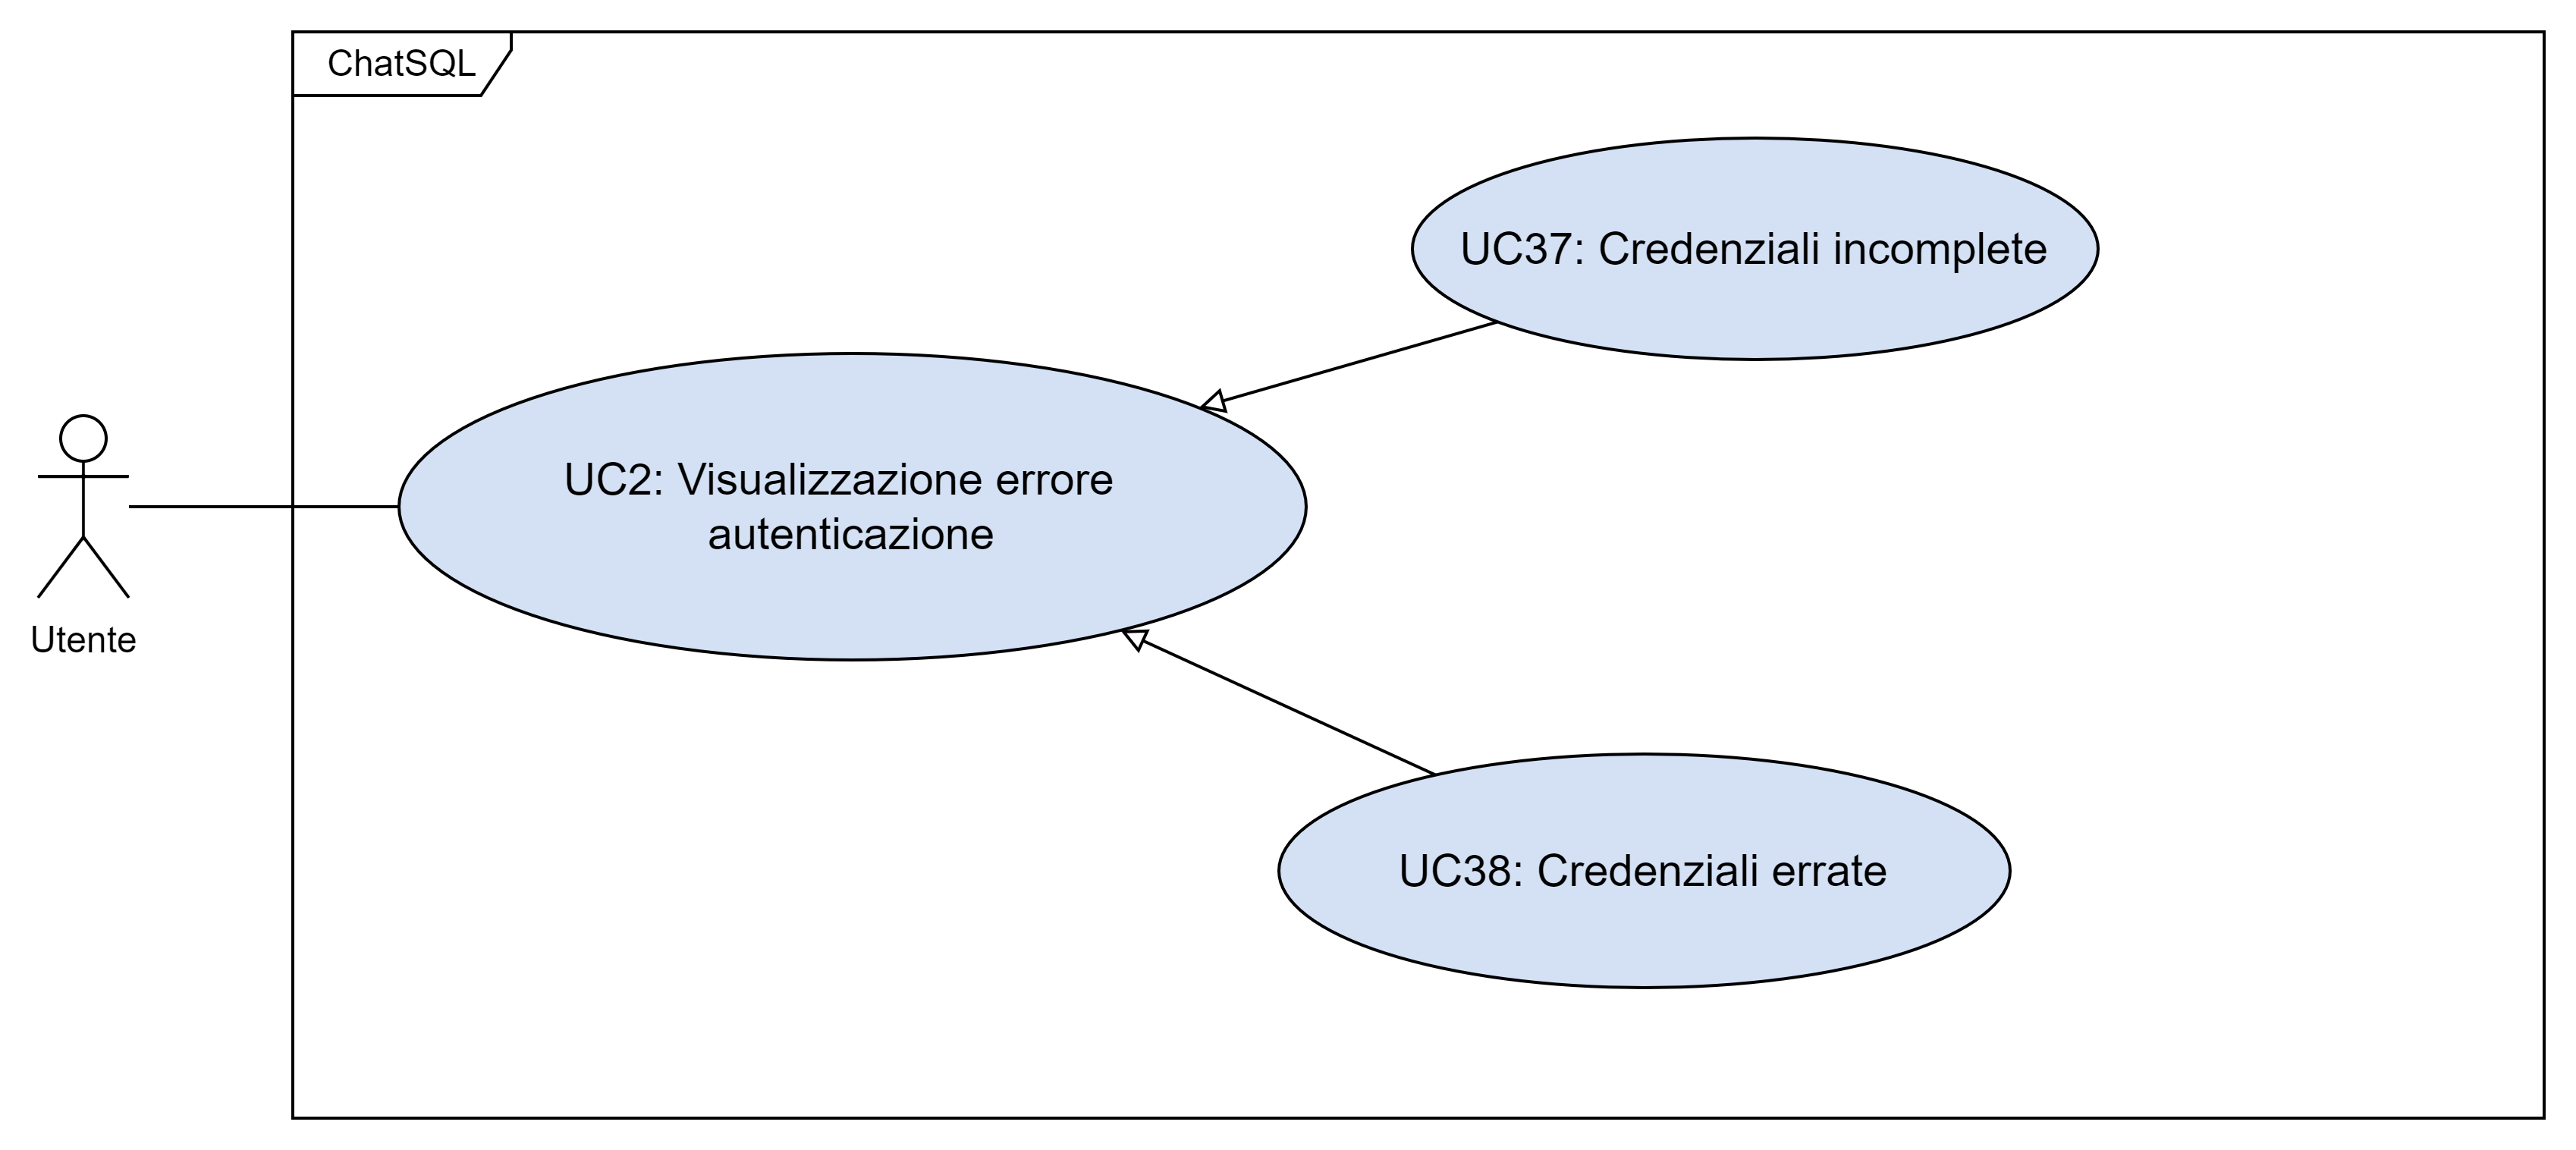
\includegraphics[width=0.90\textwidth]{assets/uc2.png}
  \caption{UC2}
\end{figure}

\paragraph*{Descrizione}
Al rilevamento da parte del sistema di irregolarità durante il processo di validazione delle credenziali al momento del login, degli appositi messaggi di errore informeranno l’Utente della natura del problema riscontrato.

\paragraph*{Attori principali}
Utente

\paragraph*{Precondizioni}
\begin{itemize}
  \item L’Utente ha inserito le proprie credenziali nell’area di login (\hyperref[UC1]{UC1});
  \item Il sistema ha riscontrato un problema nel processo di autenticazione.  
\end{itemize}

\paragraph*{Postcondizioni}
\begin{itemize}
  \item Viene mostrato un messaggio di errore per notificare l’Utente dell’incorretto o parziale inserimento dei dati nell’area di login.
\end{itemize}

\paragraph*{Scenario principale}
\begin{enumerate}
  \item L’Utente tenta di autenticarsi all’applicativo inserendo le proprie credenziali nell’area di login;
  \item Il sistema rileva lo scorretto o parziale inserimento delle credenziali;
  \item Viene segnalato all’Utente il messaggio d’errore relativo alla problematica riscontrata.  
\end{enumerate}

\paragraph*{Generalizzazioni}
\begin{itemize}
  \item Errore credenziali incomplete (\hyperref[UC2point1]{UC2.1});
  \item Errore credenziali errate (\hyperref[UC2point2]{UC2.2});
  \item Errore Utente non registrato (\hyperref[UC2point3]{UC2.3}).
\end{itemize}

%%%%%%%%%%%%%%%%%%%%%%%%%%%%%%%%%%%%%%%%%%%%%%%%%%%%%%%%%%%%%%%%%%%%%%%%%%%%%%

\subsubsection{UC2.1 - Errore credenziali incomplete}\label{UC2point1}
\paragraph*{Descrizione}
L’errore relativo all’incompletezza delle credenziali viene mostrato a seguito del rilevamento parziale delle credenziali inserite da parte dell’Utente.

\paragraph*{Attori principali}
Utente

\paragraph*{Precondizioni}
\begin{itemize}
  \item L’Utente non ha eseguito il login;
  \item L’Utente ha inserito solo il proprio username o la propria password come credenziali nel tentativo di autenticarsi.  
\end{itemize}

\paragraph*{Postcondizioni}
\begin{itemize}
  \item Viene mostrato un messaggio di errore per notificare l’Utente del parziale inserimento dei dati nell’area di login.
\end{itemize}

\paragraph*{Scenario principale}
\begin{enumerate}
  \item L’Utente ha inserito solo una delle due credenziali richieste durante il login;
  \item Il sistema mostra un messaggio di errore relativo al mancato inserimento dei dati di accesso all’applicativo.   
\end{enumerate}

%%%%%%%%%%%%%%%%%%%%%%%%%%%%%%%%%%%%%%%%%%%%%%%%%%%%%%%%%%%%%%%%%%%%%%%%%%%%%%

\subsubsection{UC2.2 - Errore credenziali errate}\label{UC2point2}
\paragraph*{Descrizione}
L’errore relativo alle credenziali errate viene mostrato in seguito all’inserimento di un username dal formato incorretto o della non corrispondenza tra username e password per un Tecnico registrato.

\paragraph*{Attori principali}
Utente

\paragraph*{Precondizioni}
\begin{itemize}
  \item L’Utente non ha eseguito il login;
  \item L’Utente ha tentato l’autenticazione con credenziali errate.  
\end{itemize}

\paragraph*{Postcondizioni}
\begin{itemize}
  \item Viene mostrato un messaggio di errore per notificare l’Utente dell’errato inserimento dei dati nell’area di login.
\end{itemize}

\paragraph*{Scenario principale}
\begin{enumerate}
  \item L’Utente ha tentato la procedura di login con credenziali errate;
  \item Il sistema mostra un messaggio di errore relativo all’errato inserimento dei dati di accesso all’applicativo.    
\end{enumerate}

%%%%%%%%%%%%%%%%%%%%%%%%%%%%%%%%%%%%%%%%%%%%%%%%%%%%%%%%%%%%%%%%%%%%%%%%%%%%%%

% Questo usercase viene modificato a seguito della presenza di una mancata corrispondenza tra username e password in UC2.2

\subsubsection{UC2.3 - Errore password errata}\label{UC2point3}
\paragraph*{Descrizione}
L’errore relativo all'inserimento di una password che non corrisponde a quella richiesta per l'accesso per l'username inserito per un Tecnico registrato.

\paragraph*{Attori principali}
Utente

\paragraph*{Precondizioni}
\begin{itemize}
  \item L’Utente non ha eseguito il login;
  \item L’Utente ha tentato l’autenticazione con un username corretto, ma una con una password errata.  
\end{itemize}

\paragraph*{Postcondizioni}
\begin{itemize}
  \item Viene mostrato un messaggio di errore per notificare l’Utente dell'inserimento di una password errata.
\end{itemize}

\paragraph*{Scenario principale}
\begin{enumerate}
  \item L’Utente ha tentato la procedura di login inserendo un username associato ad un account Tecnico, ma con una password non corrispondente per quell'utente;
  \item Il sistema mostra un messaggio di errore relativo all'inserimento errato della password.   
\end{enumerate}

\subsubsection{UC3 - Inserimento richiesta in linguaggio naturale}\label{UC3}
\paragraph*{Descrizione}
L’Utente desidera inserire una richiesta in qualsiasi linguaggio naturale al fine di ottenere il \glossario{prompt} che selezioni la parte del \glossario{dizionario dati} più inerente alla richiesta. 

\paragraph*{Attori principali}
Utente

\paragraph*{Precondizioni}
\begin{itemize}
  \item L'applicazione è stata avviata con successo;
  \item L’Utente ha in precedenza selezionato un \glossario{dizionario dati} (\hyperref[UC4]{UC4}); 
  \item L'Utente seleziona la lingua di inserimento, se non selezionata viene utilizzato l'italiano di default (\hyperref[UC7]{UC7}).
\end{itemize}

\paragraph*{Postcondizioni}
\begin{itemize}
  \item L’Utente ha scritto nell’apposito campo di testo un'interrogazione in linguaggio naturale.
\end{itemize}

\paragraph*{Scenario principale}
\begin{enumerate}
  \item L’Utente scrive un'interrogazione nell’apposito box su cui poi il sistema potrà produrre un \glossario{prompt} in seguito.
\end{enumerate}

\subsubsection{UC4 - Selezione \glossario{dizionario dati}}\label{UC4}

\begin{figure}[H]
  \centering
  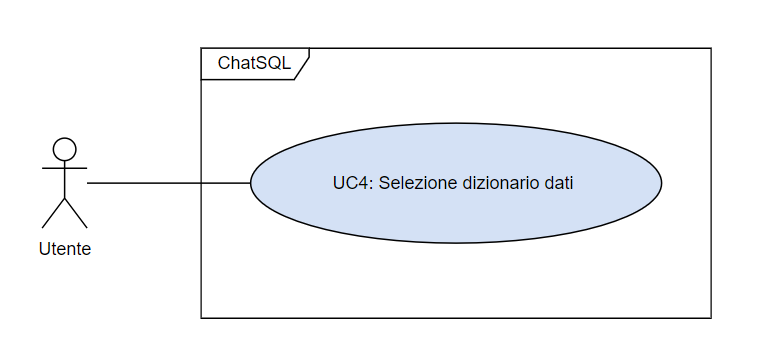
\includegraphics[width=0.90\textwidth]{assets/uc4.png}
  \caption{UC4}
\end{figure}

\paragraph*{Descrizione}
L’Utente desidera selezionare il \glossario{dizionario dati} sul quale basare in seguito l’interrogazione in linguaggio naturale.

\paragraph*{Attori principali}
Utente

\paragraph*{Precondizioni}
\begin{itemize}
  \item L'applicazione è stata avviata con successo;
  \item Nell'applicazione web è stato caricato precedentemente almeno un \glossario{dizionario dati} (\hyperref[UC13]{UC13}).
\end{itemize}

\paragraph*{Postcondizioni}
\begin{itemize}
  \item Un \glossario{dizionario dati} è stato selezionato in modo corretto ed univoco.
\end{itemize}

\paragraph*{Scenario principale}
\begin{enumerate}
  \item L’Utente visualizza la lista dei dizionari disponibili (\hyperref[UC10]{UC10});
  \item L'Utente sceglie un \glossario{dizionario dati} tra quelli presenti.
\end{enumerate}

% Da inserire caso d'errore per l'indisponibilità del dizionario dati
\subsubsection{UC5 - Generazione prompt}\label{UC5}
\paragraph*{Descrizione}
L’Utente desidera ottenere un prompt al fine di utilizzarlo poi con LLM esterni per generare \glossario{query} sql fornendo parti ristrette di \glossario{dizionario dati}.

\paragraph*{Attori principali}
Utente

\paragraph*{Precondizioni}
\begin{itemize}
  \item L'applicazione è stata avviata con successo;
  \item È presente almeno un \glossario{dizionario dati} nel sistema.
\end{itemize}

\paragraph*{Postcondizioni}
\begin{itemize}
  \item Il sistema genera un prompt in base alla richiesta ricevuta e al \glossario{dizionario dati} scelto. Attraverso dei metadati restituisce un prompt con il quale stabilisce quali parti di database sono maggiormente necessarie ed efficienti per scrivere la richiesta ricevuta in SQL;
  \item L’Utente riceve il prompt generato.
\end{itemize}

\paragraph*{Scenario principale}
\begin{enumerate}
  \item L’Utente desidera ottenere il prompt che permette di generare la query SQL;
  \item L’Utente seleziona un \glossario{dizionario dati} sul quale baserà l’interrogazione;
  \item L’Utente sceglie la lingua su cui farà l’interrogazione.La lingua è in italiano di default se non viene cambiata;
  \item L’Utente inserisce una interrogazione in linguaggio naturale nel box testuale apposito;
  \item Inizia il processo di generazione del prompt e di raccolta di metadati.
\end{enumerate}

\paragraph*{Scenario alternativo}
\begin{enumerate}
  \item Errore nella generazione del prompt (\hyperref[UC6]{UC6}).
\end{enumerate}

\paragraph*{Inclusione}
\begin{itemize}
  \item Inserimento richiesta in linguaggio naturale (\hyperref[UC3]{UC3});
  \item Selezione \glossario{dizionario dati} (\hyperref[UC4]{UC4}).
\end{itemize}

\paragraph*{Estensione}
\begin{itemize}
  \item Cambio lingua (\hyperref[UC7]{UC7});
  \item Selezione e copia del prompt risultato (\hyperref[UC8]{UC8}).
\end{itemize}

\subsubsection{UC6 - Richiesta non idonea}\label{UC6}
\paragraph*{Descrizione}
Nel caso in cui l'Utente formuli una richiesta non idonea, o comunque una frase che non trova corrispondenze con il \glossario{dizionario dati}, il sistema restituisce un messaggio notificando l'Utente della mancata generazione del \glossario{prompt}.

\paragraph*{Attori principali}
Utente

\paragraph*{Precondizioni}
\begin{itemize}
  \item L'applicazione è stata avviata con successo;
  \item Nel sistema è stato caricato almeno un \glossario{dizionario dati};
  \item L'Utente ha richiesto la generazione del \glossario{prompt} (\hyperref[UC5]{UC5}).  
\end{itemize}

\paragraph*{Postcondizioni}
\begin{itemize}
  \item Viene visualizzato correttamente il messaggio del ChatBOT, che avvisa l'Utente della mancata generazione del \glossario{prompt}.
\end{itemize}

\paragraph*{Scenario principale}
\begin{enumerate}
  \item Il sistema è attivo e funzionante;
  \item L'Utente richiede la generazione del \glossario{prompt} (\hyperref[UC5]{UC5});
  \item Il sistema non trova correlazioni tra la richiesta dell'Utente e il \glossario{dizionario dati};
  \item Il sistema non è in grado restituire un \glossario{prompt} adeguato alla richiesta dell'Utente;
  \item Viene visualizzato un messaggio che informa l'Utente dell'esito negativo della ricerca semantica e lo invita a riprovare.
\end{enumerate}

\subsubsection{UC7 - Cambio lingua}\label{UC7}
\paragraph*{Descrizione}
L’Utente desidera inserire una richiesta in linguaggio naturale in una lingua diversa dall’italiano.

\paragraph*{Attori principali}
Utente

\paragraph*{Precondizioni}
\begin{itemize}
  \item L'applicazione è stata avviata con successo;
  \item L’Utente vuole inserire una frase in linguaggio naturale in un'altra lingua.
\end{itemize}

\paragraph*{Postcondizioni}
\begin{itemize}
  \item L'Utente ha selezionato una lingua tra quelle disponibili;
  \item L'Utente inserisce una richiesta in linguaggio naturale nella lingua scelta (\hyperref[UC3]{UC3});
  \item L'applicazione opera la generazione del \glossario{prompt} considerando la lingua selezionata (\hyperref[UC5]{UC5}).
\end{itemize}

\paragraph*{Scenario principale}
\begin{enumerate}
  \item L’Utente seleziona una lingua da una lista predefinita di lingue. La scelta è tra:
    \begin{itemize}
      \item Italiano;
      \item Inglese;
      \item Francese;
      \item Spagnolo;
      \item Tedesco.
    \end{itemize}
  \item L’Utente inserisce una interrogazione in linguaggio naturale nella lingua selezionata (\hyperref[UC3]{UC3}).  
\end{enumerate}

% TODO [in caso di errore ed incongruenza tra la lingua scritta e quella selezionata teniamo solo errore uc6 del \glossario{prompt}? O viene controllata prima?]

\subsubsection{UC8 - Copia del \glossario{prompt} generato}\label{UC8}

\begin{figure}[H]
  \centering
  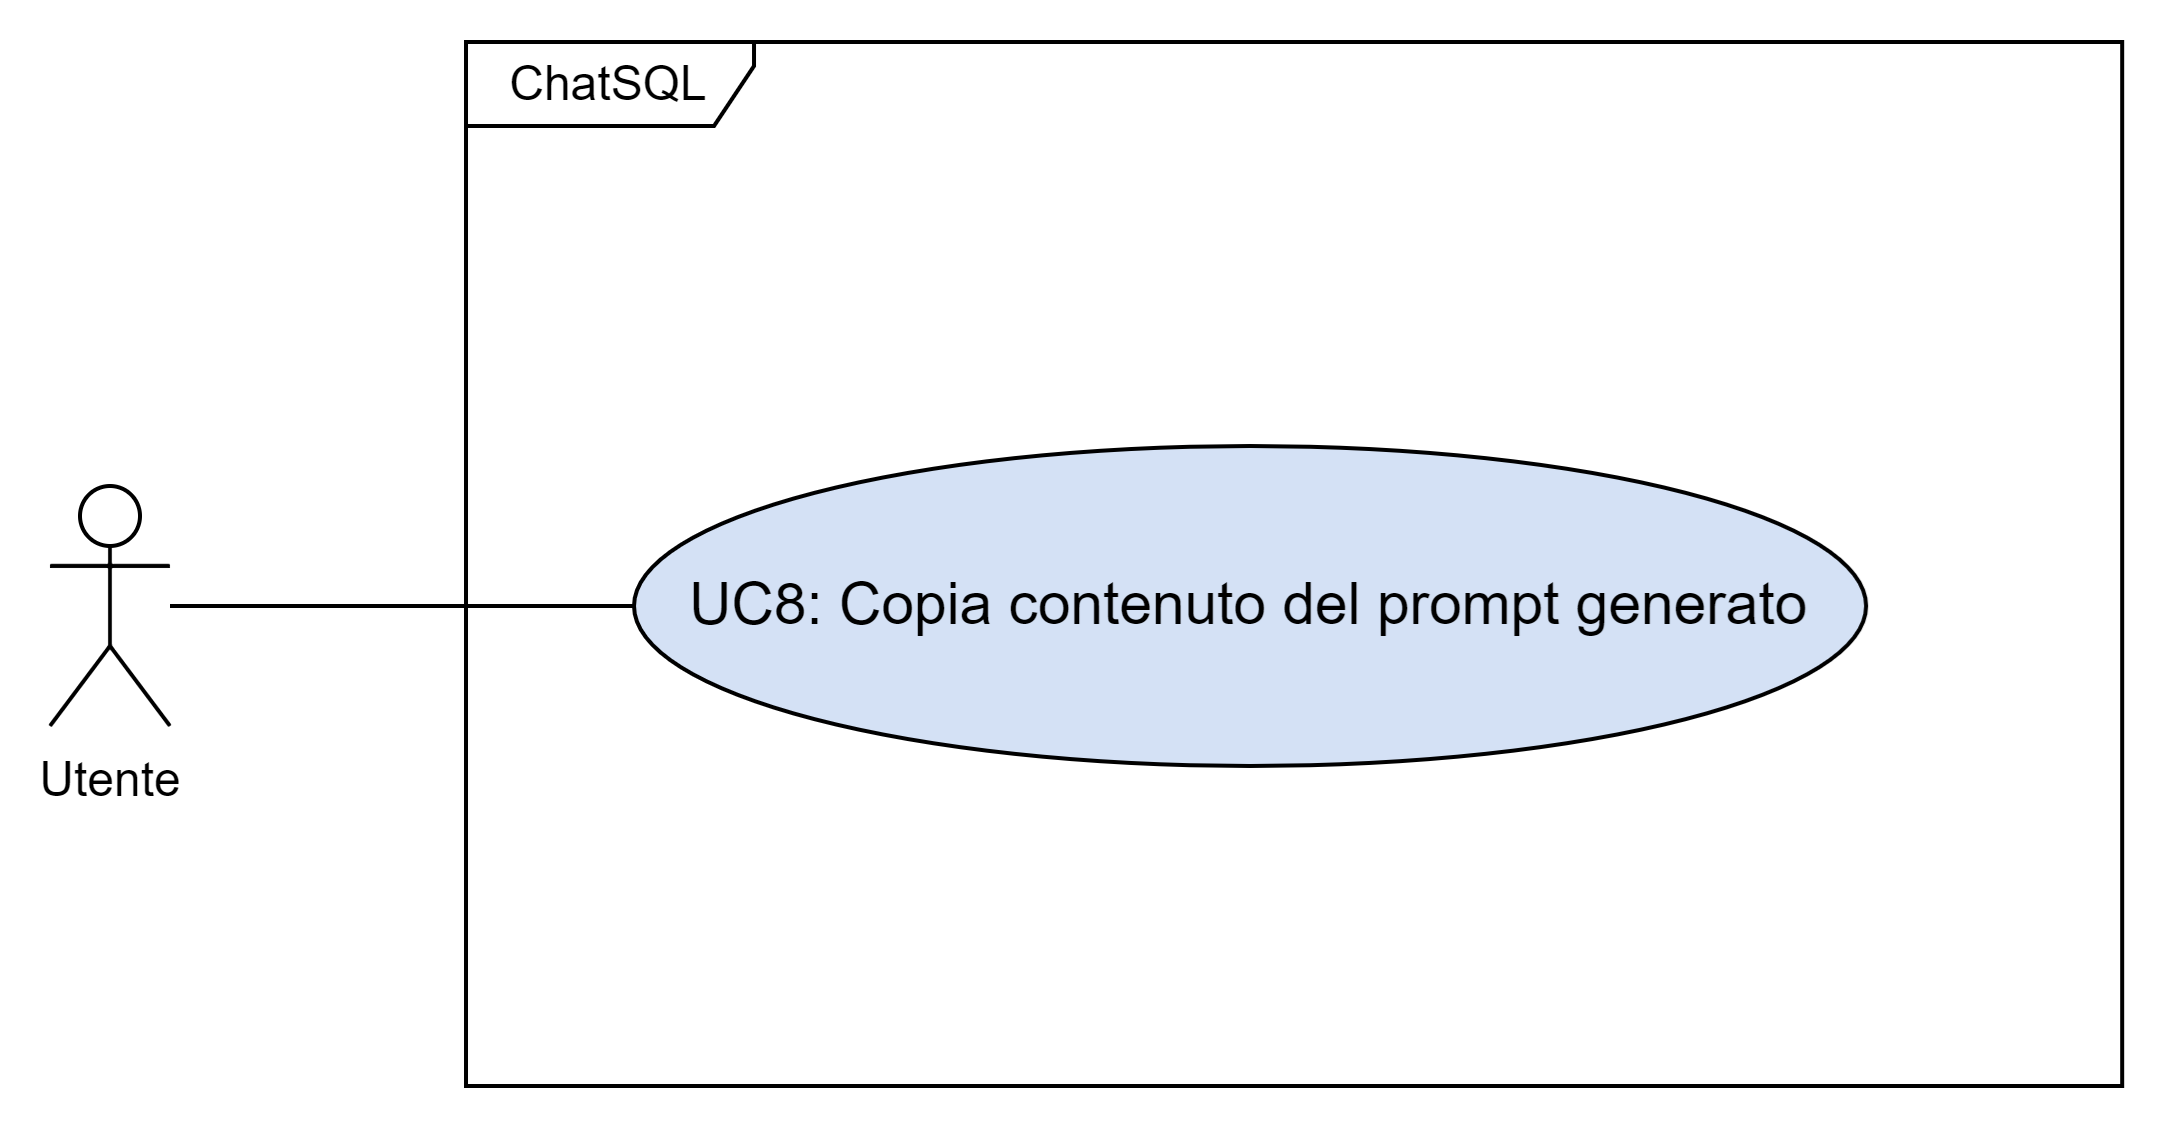
\includegraphics[width=0.90\textwidth]{assets/uc8.png}
  \caption{UC8}
\end{figure}

\paragraph*{Descrizione}
L'Utente può copiare il contenuto del \glossario{prompt} negli appunti di sistema, per poi incollarlo agevolmente in un servizio esterno.

\paragraph*{Attori principali}
Utente

\paragraph*{Precondizioni}
\begin{itemize}
  \item L'applicazione è stata avviata con successo;
  \item Il sistema ha generato almeno un \glossario{prompt}.  
\end{itemize}

\paragraph*{Postcondizioni}
\begin{itemize}
  \item Il \glossario{prompt} viene correttamente copiato negli appunti di sistema dell'Utente.
\end{itemize}

\paragraph*{Trigger}
L'Utente desidera copiare il \glossario{prompt} generato, con l'obiettivo di effettuare un'operazione di "Copy and Paste", incollando il contenuto del prompt in un servizio esterno che implementi \glossario{LLM}.

\paragraph*{Scenario principale}
\begin{enumerate}
  \item L'Utente visualizza il \glossario{prompt} generato;
  \item L'Utente seleziona la funzione di copia;
  \item Negli appunti di sistema viene salvata una copia del \glossario{prompt}, che può essere fornita in input a un \glossario{LLM} esterno per la generazione di una \glossario{query} SQL.
\end{enumerate}
\subsubsection{UC9 - Visualizzazione lista dizionari dati caricati nel sistema}\label{UC9}

\begin{figure}[H]
  \centering
  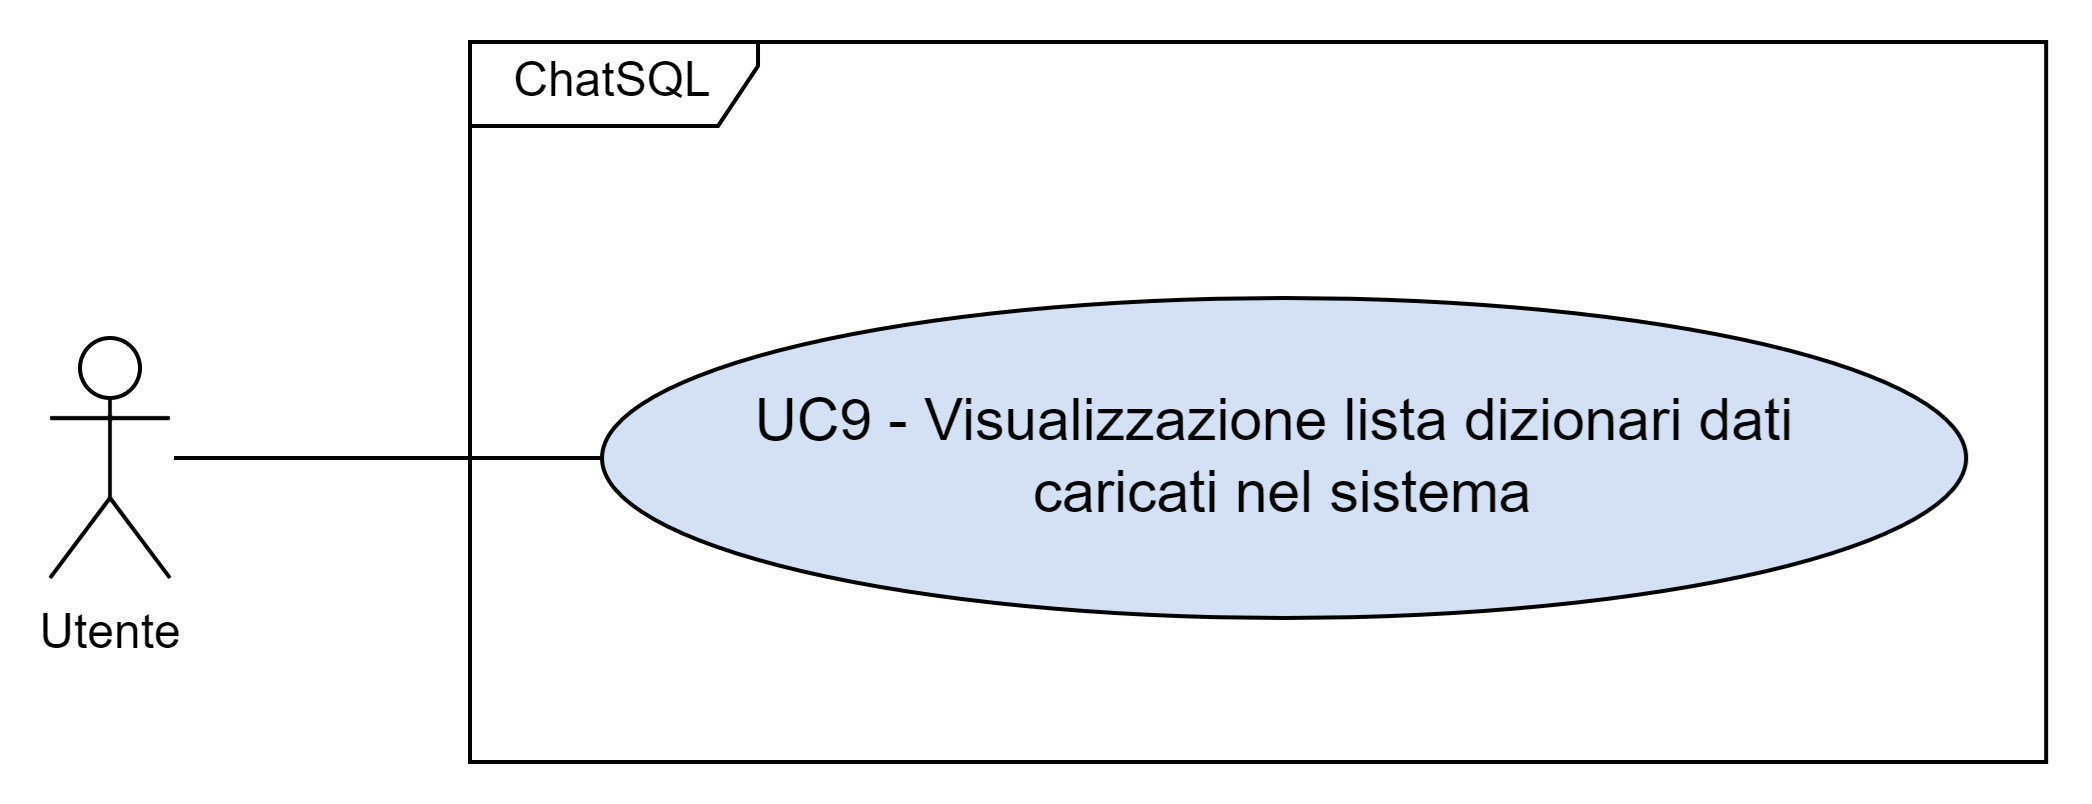
\includegraphics[width=0.90\textwidth]{assets/uc9.png}
  \caption{UC9}
\end{figure}

\paragraph*{Descrizione}
L'Utente visualizza la lista dei \glossario{dizionari dati} che sono stati caricati nel sistema.

\paragraph*{Attori principali}
Utente

\paragraph*{Precondizioni}
\begin{itemize}
  \item Il sistema è attivo e funzionante;
  \item È stato caricato almeno un \glossario{dizionario dati}.  
\end{itemize}

\paragraph*{Postcondizioni}
\begin{itemize}
\item Viene visualizzata la lista dei \glossario{dizionari dati} presenti nel sistema.
\end{itemize}

\paragraph*{Trigger}
L'Utente desidera visualizzare i \glossario{dizionari dati} disponibili.

\paragraph*{Scenario principale}
\begin{enumerate}
  \item L'Utente visualizza la lista dei \glossario{dizionari dati}.
\end{enumerate}

\paragraph*{Sottocasi d'uso:}
\begin{enumerate}
  \item \hyperref[UC9point1]{UC9.1}: Visualizzazione singolo dizionario dati.
\end{enumerate}

\begin{figure}[H]
  \centering
  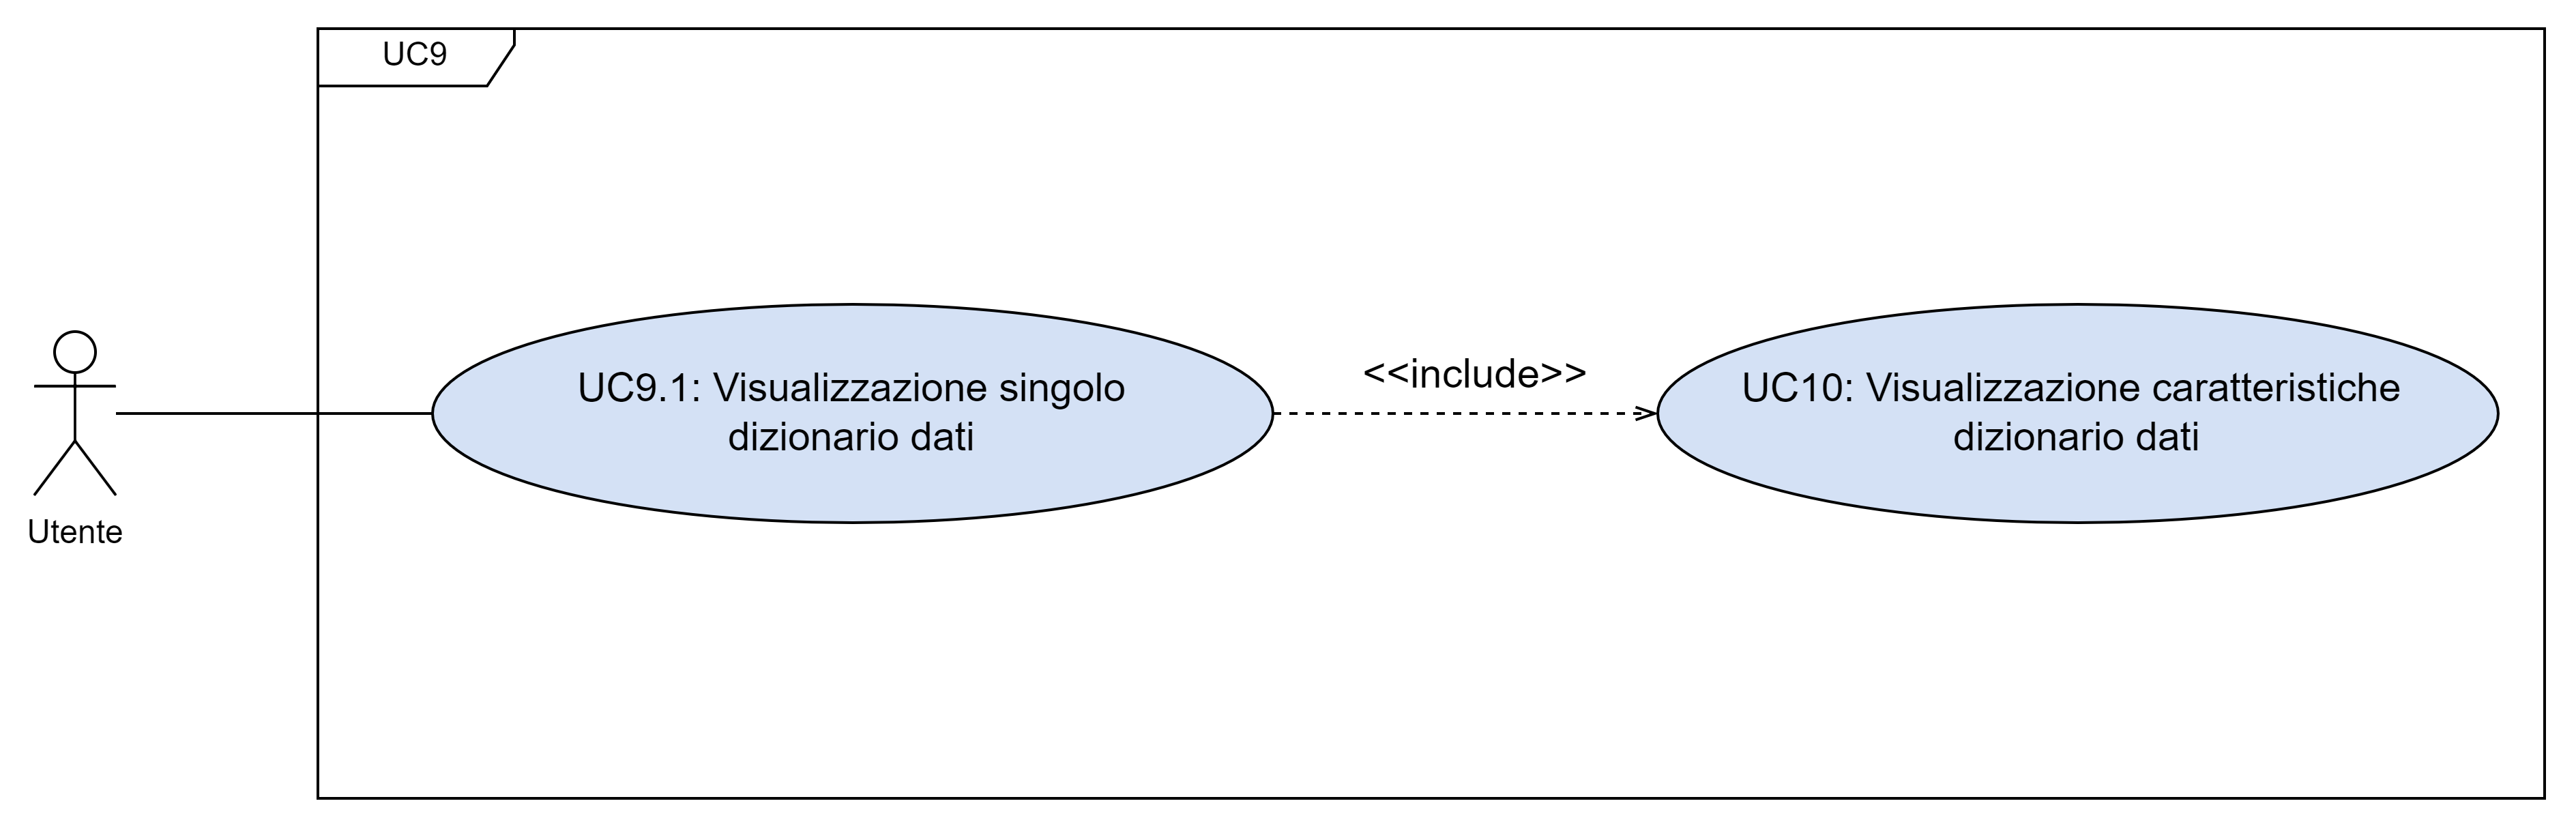
\includegraphics[width=0.90\textwidth]{assets/uc9_1.png}
  \caption{UC9 - Sottocasi d'uso}
\end{figure}

%%%%%%%%%%%%%%%%%%%%%%%%%%%%%%%%%%%%%%%%%%%%%%%%%%%%%%%%%%%%%%%%%%%%%%%%%%%%%%

\subsubsection{UC9.1 - Visualizzazione singolo dizionario dati}\label{UC9point1}
\paragraph*{Descrizione}
L'Utente visualizza un dizionario all'interno della lista dei \glossario{dizionari dati} caricati nel sistema.

\paragraph*{Attori principali}
Utente

\paragraph*{Precondizioni}
\begin{itemize}
  \item Il sistema è attivo e funzionante;
  \item È stato caricato almeno un dizionario dati;
  \item È visibile la lista dei \glossario{dizionari dati} (\hyperref[UC9]{UC9}).
\end{itemize}

\paragraph*{Postcondizioni}
\begin{itemize}
  \item Viene visualizzato correttamente il \glossario{dizionario dati}.
\end{itemize}

\paragraph*{Trigger}
L'Utente desidera visualizzare un dizionario all'interno della lista.

\paragraph*{Scenario principale}
\begin{enumerate}
  \item L'Utente visualizza un singolo \glossario{dizionario dati}.
\end{enumerate}

\paragraph*{Inclusioni}
\begin{itemize}
  \item Visualizzazione caratteristiche dizionario dati (\hyperref[UC10]{UC10}).
\end{itemize}
\subsubsection{UC10 - Visualizzazione caratteristiche dizionario dati}\label{UC10}
\paragraph*{Descrizione}
Il sistema mostra le caratteristiche del \glossario{dizionario dati}.

\paragraph*{Attori principali}
Utente

\paragraph*{Precondizioni}
\begin{itemize}
  \item Il sistema è attivo e funzionante;
  \item È stato caricato almeno un \glossario{dizionario dati} nel sistema.  
\end{itemize}

\paragraph*{Postcondizioni}
\begin{itemize}
  \item Vengono visualizzate correttamente le caratteristiche del \glossario{dizionario dati}.
\end{itemize}

\paragraph*{Trigger}
L'Utente vuole visualizzare le caratteristiche di un \glossario{dizionario dati}.

\paragraph*{Scenario principale}
\begin{enumerate}
  \item L'Utente visualizza le caratteristiche del \glossario{dizionario dati}.
\end{enumerate}

\begin{figure}[H]
  \centering
  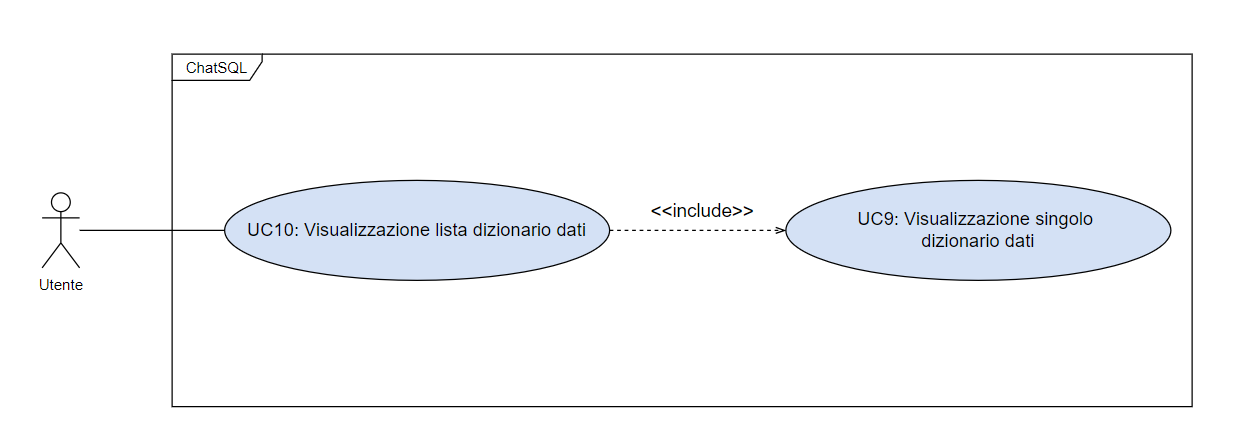
\includegraphics[width=0.90\textwidth]{assets/uc10.png}
  \caption{UC10 - Sottocasi d'uso}
\end{figure}

%%%%%%%%%%%%%%%%%%%%%%%%%%%%%%%%%%%%%%%%%%%%%%%%%%%%%%%%%%%%%%%%%%%%%%%%%%%%%%

\subsubsection{UC10.1 - Visualizzazione nome dizionario dati}\label{UC10point1}
\paragraph*{Descrizione}
L'Utente visualizza il nome del \glossario{dizionario dati}.

\paragraph*{Attori principali}
Utente

\paragraph*{Precondizioni}
\begin{itemize}
  \item Il sistema è attivo e funzionante;
  \item È stato caricato almeno un \glossario{dizionario dati} nel sistema. 
\end{itemize}

\paragraph*{Postcondizioni}
\begin{itemize}
  \item Viene visualizzato correttamente il nome del \glossario{dizionario dati}.
\end{itemize}

\paragraph*{Trigger}
L'Utente vuole visualizzare il nome di un \glossario{dizionario dati}.

\paragraph*{Scenario principale}
\begin{enumerate}
  \item L'Utente visualizza il nome del \glossario{dizionario dati}.
\end{enumerate}

%%%%%%%%%%%%%%%%%%%%%%%%%%%%%%%%%%%%%%%%%%%%%%%%%%%%%%%%%%%%%%%%%%%%%%%%%%%%%%

\subsubsection{UC10.2 - Visualizzazione estensione dizionario dati}\label{UC10point2}
\paragraph*{Descrizione}
L'Utente visualizza l'estensione del \glossario{dizionario dati} (es.: .json, .sql).

\paragraph*{Attori principali}
Utente

\paragraph*{Precondizioni}
\begin{itemize}
  \item Il sistema è attivo e funzionante;
  \item È stato caricato almeno un \glossario{dizionario dati} nel sistema. 
\end{itemize}

\paragraph*{Postcondizioni}
\begin{itemize}
  \item Viene visualizzata correttamente l'estensione del \glossario{dizionario dati}.
\end{itemize}

\paragraph*{Trigger}
L'Utente vuole visualizzare l'estensione di un \glossario{dizionario dati}.

\paragraph*{Scenario principale}
\begin{enumerate}
  \item L'Utente visualizza l'estensione del \glossario{dizionario dati}.
\end{enumerate}

%%%%%%%%%%%%%%%%%%%%%%%%%%%%%%%%%%%%%%%%%%%%%%%%%%%%%%%%%%%%%%%%%%%%%%%%%%%%%%

\subsubsection{UC10.3 - Visualizzazione descrizione dizionario dati}\label{UC10point3}
\paragraph*{Descrizione}
L'Utente visualizza la descrizione del \glossario{dizionario dati}.

\paragraph*{Attori principali}
Utente

\paragraph*{Precondizioni}
\begin{itemize}
  \item Il sistema è attivo e funzionante;
  \item È stato caricato almeno un \glossario{dizionario dati} nel sistema. 
\end{itemize}

\paragraph*{Postcondizioni}
\begin{itemize}
  \item Viene visualizzata correttamente la descrizione del \glossario{dizionario dati}.
\end{itemize}

\paragraph*{Trigger}
L'Utente vuole visualizzare la descrizione di un \glossario{dizionario dati}.

\paragraph*{Scenario principale}
\begin{enumerate}
  \item L'Utente visualizza la descrizione del \glossario{dizionario dati}.
\end{enumerate}

%%%%%%%%%%%%%%%%%%%%%%%%%%%%%%%%%%%%%%%%%%%%%%%%%%%%%%%%%%%%%%%%%%%%%%%%%%%%%%

\subsubsection{UC10.4 - Visualizzazione dimensione dizionario dati}\label{UC10point4}
\paragraph*{Descrizione}
L'Utente visualizza la dimensione del \glossario{dizionario dati}, che corrisponde al peso del file (es.: 500 KB).

\paragraph*{Attori principali}
Utente

\paragraph*{Precondizioni}
\begin{itemize}
  \item Il sistema è attivo e funzionante;
  \item È stato caricato almeno un \glossario{dizionario dati} nel sistema. 
\end{itemize}

\paragraph*{Postcondizioni}
\begin{itemize}
  \item Viene visualizzata correttamente la dimensione del \glossario{dizionario dati}.
\end{itemize}

\paragraph*{Trigger}
L'Utente vuole visualizzare la dimensione di un \glossario{dizionario dati}.

\paragraph*{Scenario principale}
\begin{enumerate}
  \item L'Utente visualizza la dimensione del \glossario{dizionario dati}.
\end{enumerate}

%%%%%%%%%%%%%%%%%%%%%%%%%%%%%%%%%%%%%%%%%%%%%%%%%%%%%%%%%%%%%%%%%%%%%%%%%%%%%%

\subsubsection{UC10.5 - Visualizzazione data di ultimo aggiornamento dizionario dati}\label{UC10point5}
\paragraph*{Descrizione}
L'Utente visualizza la data di ultimo aggiornamento del \glossario{dizionario dati}.

\paragraph*{Attori principali}
Utente

\paragraph*{Precondizioni}
\begin{itemize}
  \item Il sistema è attivo e funzionante;
  \item È stato caricato almeno un \glossario{dizionario dati} nel sistema. 
\end{itemize}

\paragraph*{Postcondizioni}
\begin{itemize}
  \item Viene visualizzata correttamente la data di ultimo aggiornamento del \glossario{dizionario dati}.
\end{itemize}

\paragraph*{Trigger}
L'Utente vuole visualizzare la data di ultimo aggiornamento di un \glossario{dizionario dati}.

\paragraph*{Scenario principale}
\begin{enumerate}
  \item L'Utente visualizza la data di ultimo aggiornamento del \glossario{dizionario dati}.
\end{enumerate}
\subsubsection{UC11 - Messaggio errore fallimento caricamento \glossario{dizionario dati}}\label{UC11}
\paragraph*{Descrizione}
L’Utente visualizza il messaggio di errore che informa del fallimento del caricamento dei dizionari dati.

\paragraph*{Attori principali}
Utente

\paragraph*{Precondizioni}
\begin{itemize}
  \item L’Utente è stato autenticato con successo;
  \item Esiste almeno un \glossario{dizionario dati} caricato.  
\end{itemize}

\paragraph*{Postcondizioni}
\begin{itemize}
  \item Viene mostrato il messaggio di errore.
\end{itemize}

\paragraph*{Scenario principale}
\begin{enumerate}
  \item L’Utente accede alla modalità di visualizzazione della lista dei dizionari dati;
  \item Il sistema non è in grado di elaborare la richiesta;
  \item Viene presentato il messaggio d’errore corrispondente al tipo del problema.  
\end{enumerate}

\subsubsection{UC12 - Logout}\label{UC12}
\paragraph*{Descrizione}
Un Utente può disconnettersi dalla piattaforma tramite la procedura di logout.

\paragraph*{Attori principali}
Utente

\paragraph*{Precondizioni}
\begin{itemize}
  \item L’Utente è correttamente autenticato. 
\end{itemize}

\paragraph*{Postcondizioni}
\begin{itemize}
  \item L’Utente ha eseguito il logout e non ha più accesso alle funzionalità base dell’applicativo.
\end{itemize}

\paragraph*{Scenario principale}
\begin{enumerate}
  \item L’Utente desidera terminare la sessione corrente e clicca sul tasto di logout;
  \item La sessione dell’Utente viene terminata.  
\end{enumerate}

\subsubsection{UC13 - Salvataggio di un dizionario dati nel sistema}\label{UC13}

\begin{figure}[H]
  \centering
  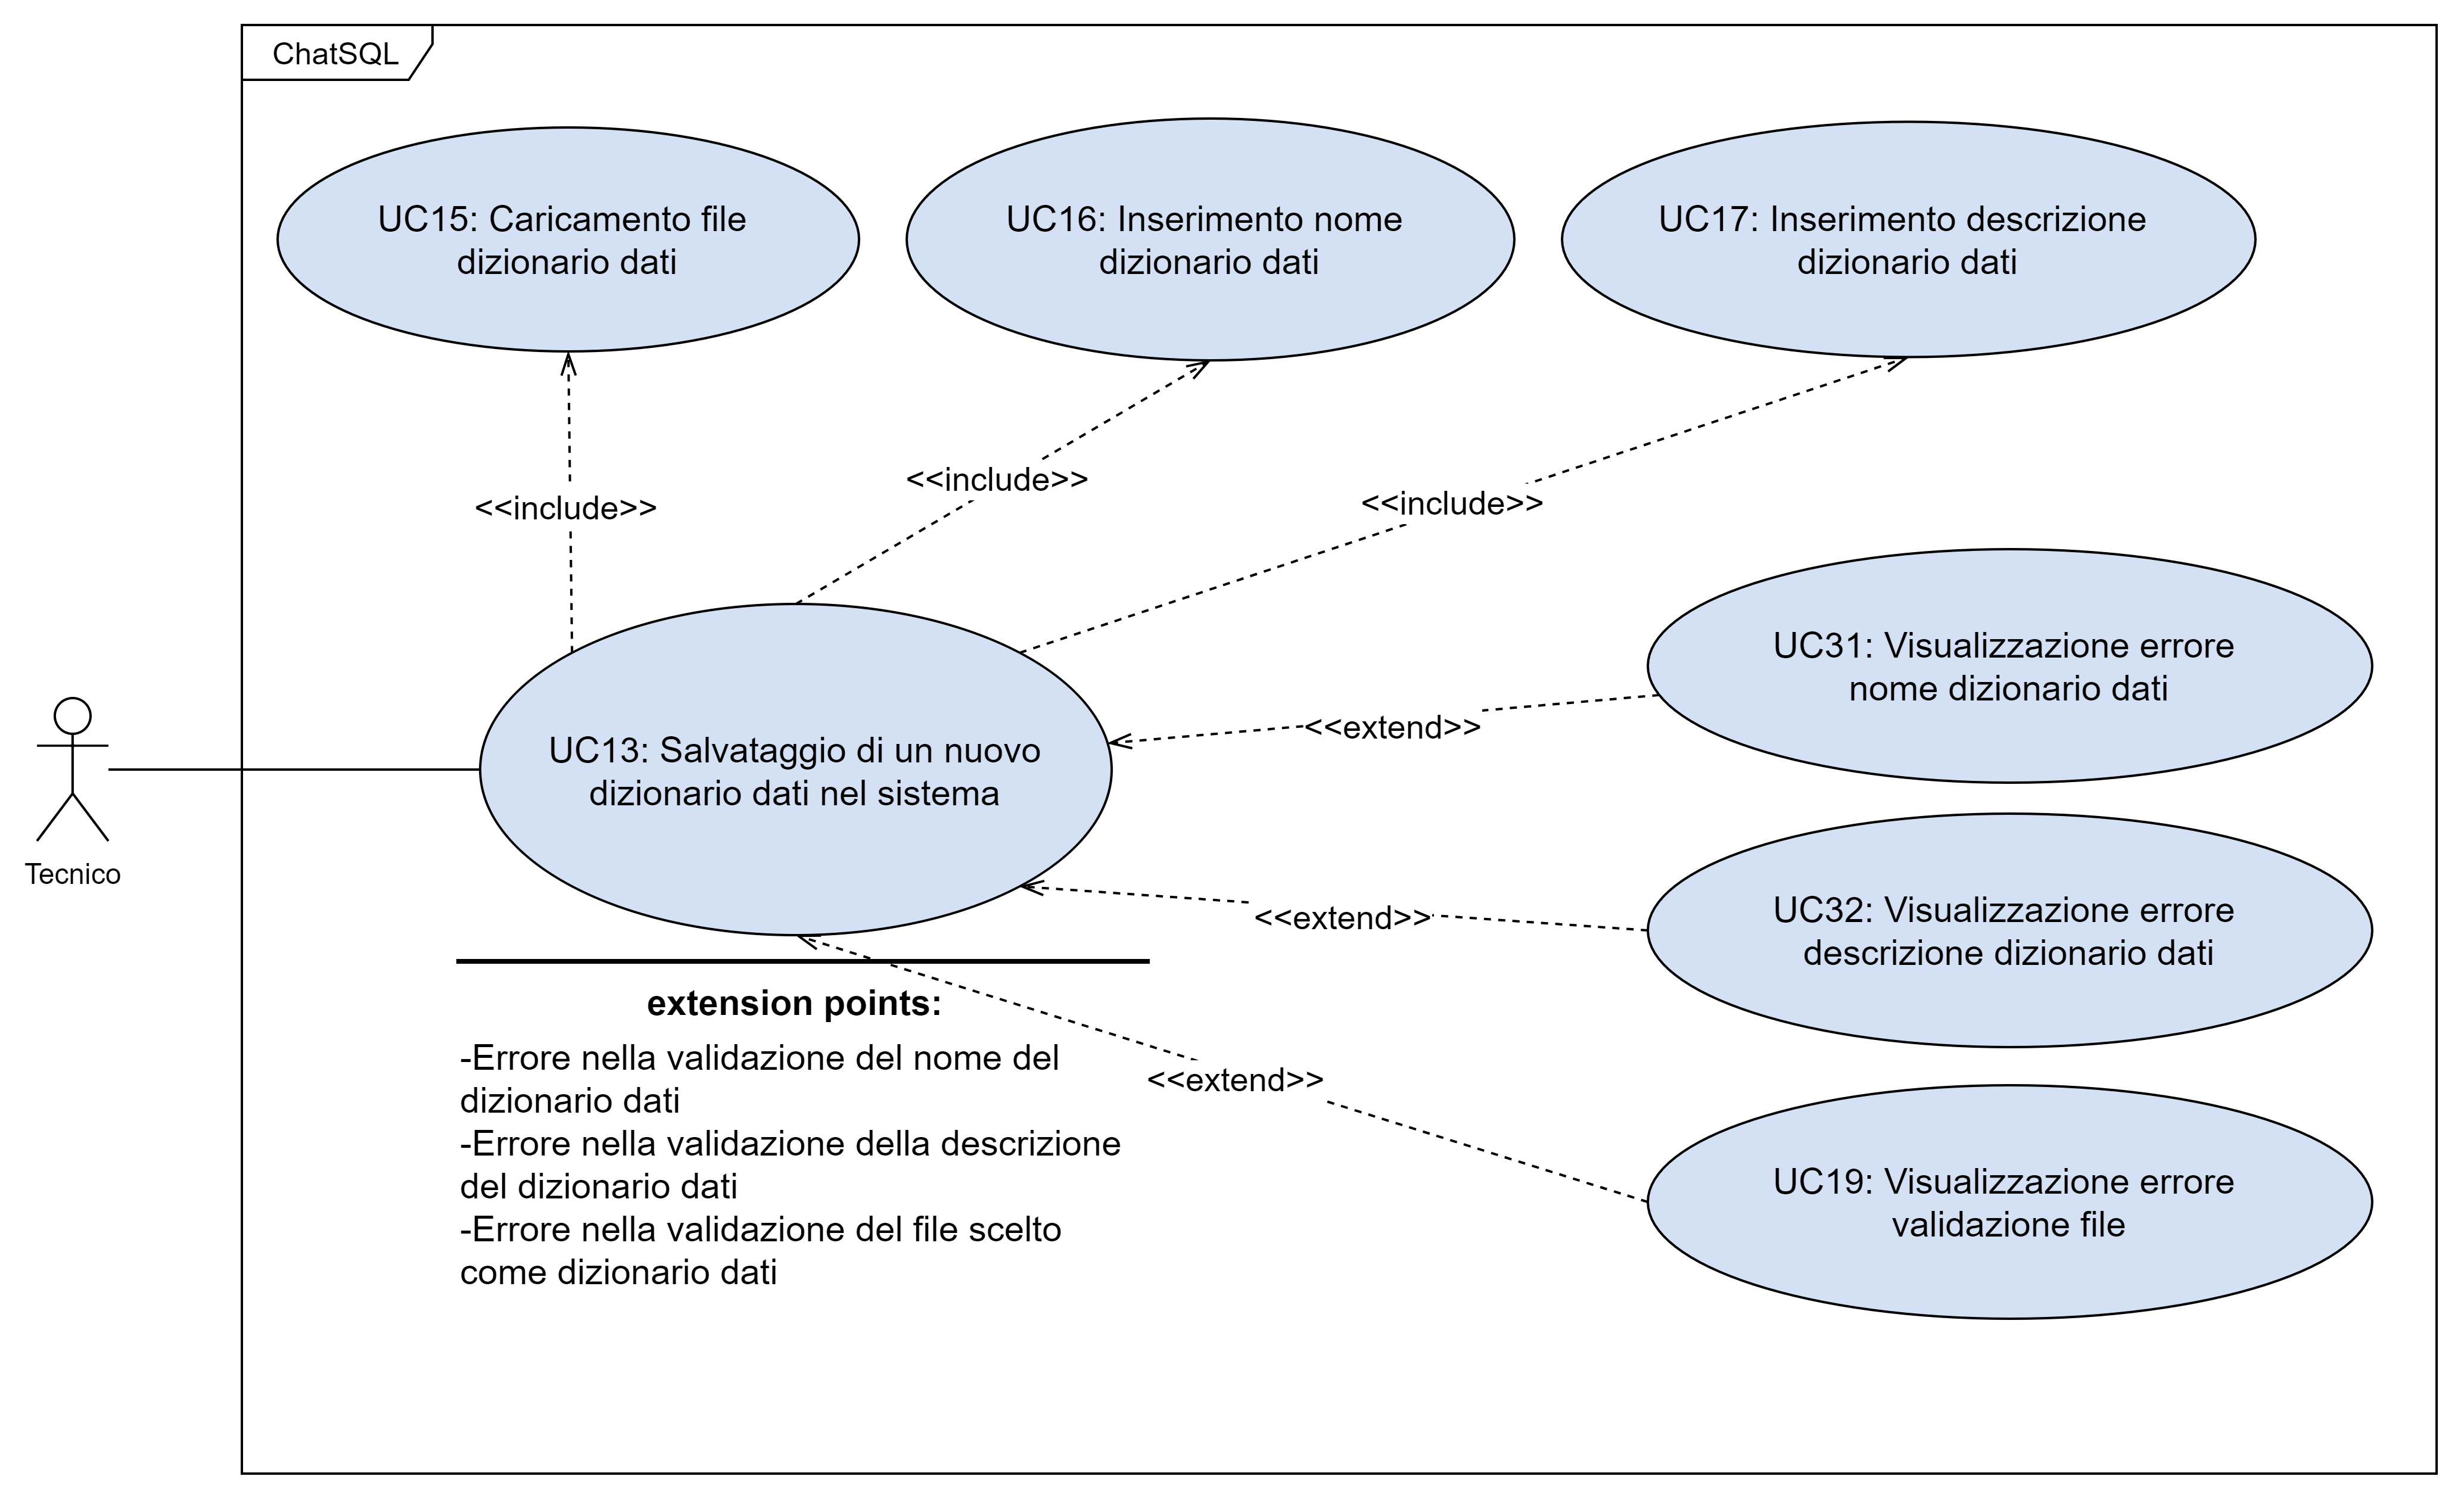
\includegraphics[width=0.90\textwidth]{assets/uc13.png}
  \caption{UC13}
\end{figure}

\paragraph*{Descrizione}
Il salvataggio di un \glossario{dizionario dati} corrisponde alla procedura di inserimento di un dizionario e delle sue informazioni all'interno del sistema.

\paragraph*{Attori principali}
Tecnico

\paragraph*{Precondizioni}
\begin{itemize}
  \item Il sistema è attivo e funzionante;
  \item Il Tecnico ha effettuato l'autenticazione (\hyperref[UC1]{UC1});
\end{itemize}

\paragraph*{Postcondizioni}
\begin{itemize}
  \item Il \glossario{dizionario dati} è stato salvato con successo.
\end{itemize}

\paragraph*{Trigger}
Il Tecnico vuole aggiungere un nuovo \glossario{dizionario dati} nell'applicazione.

\paragraph*{Scenario principale}
\begin{enumerate}
  \item Il Tecnico inserisce il file, il nome e la descrizione del \glossario{dizionario dati};
  \item Il Tecnico richiede il salvataggio del \glossario{dizionario dati};
  \item Il \glossario{dizionario dati} viene salvato nel sistema;
  \item Il \glossario{dizionario dati} è disponibile a tutti gli utenti;
  \item Il \glossario{dizionario dati} può essere utilizzato per la generazione di \glossario{prompt}.
\end{enumerate}

\paragraph*{Scenario alternativo}
\begin{enumerate}
  \item Il sistema riscontra un errore durante la validazione del \glossario{dizionario dati};
  \item Viene visualizzato un messaggio d'errore esplicativo.
\end{enumerate}

\paragraph*{Inclusioni}
\begin{itemize}
  \item Caricamento file dizionario dati (\hyperref[UC15]{UC15});
  \item Inserimento nome dizionario dati (\hyperref[UC16]{UC16});
  \item Inserimento descrizione dizionario dati (\hyperref[UC17]{UC17}).
\end{itemize}

\paragraph*{Estensioni}
\begin{itemize}
  \item Visualizzazione errore validazione file (\hyperref[UC19]{UC19}).
  \begin{itemize}
    \item Extension point: errore nella validazione del file scelto come \glossario{dizionario dati}.
  \end{itemize}
  \item Visualizzazione errore nome \glossario{dizionario dati} (\hyperref[UC31]{UC31}).
  \begin{itemize}
    \item Extension point: errore nella validazione del nome del \glossario{dizionario dati}.
  \end{itemize}
  \item Visualizzazione errore descrizione \glossario{dizionario dati} (\hyperref[UC32]{UC32}).
  \begin{itemize}
    \item Extension point: errore nella validazione della descrizione del \glossario{dizionario dati}.
  \end{itemize}
\end{itemize}

\subsubsection{UC14 - Visualizzazione contenuto dizionario dati}\label{UC14}

\begin{figure}[H]
  \centering
  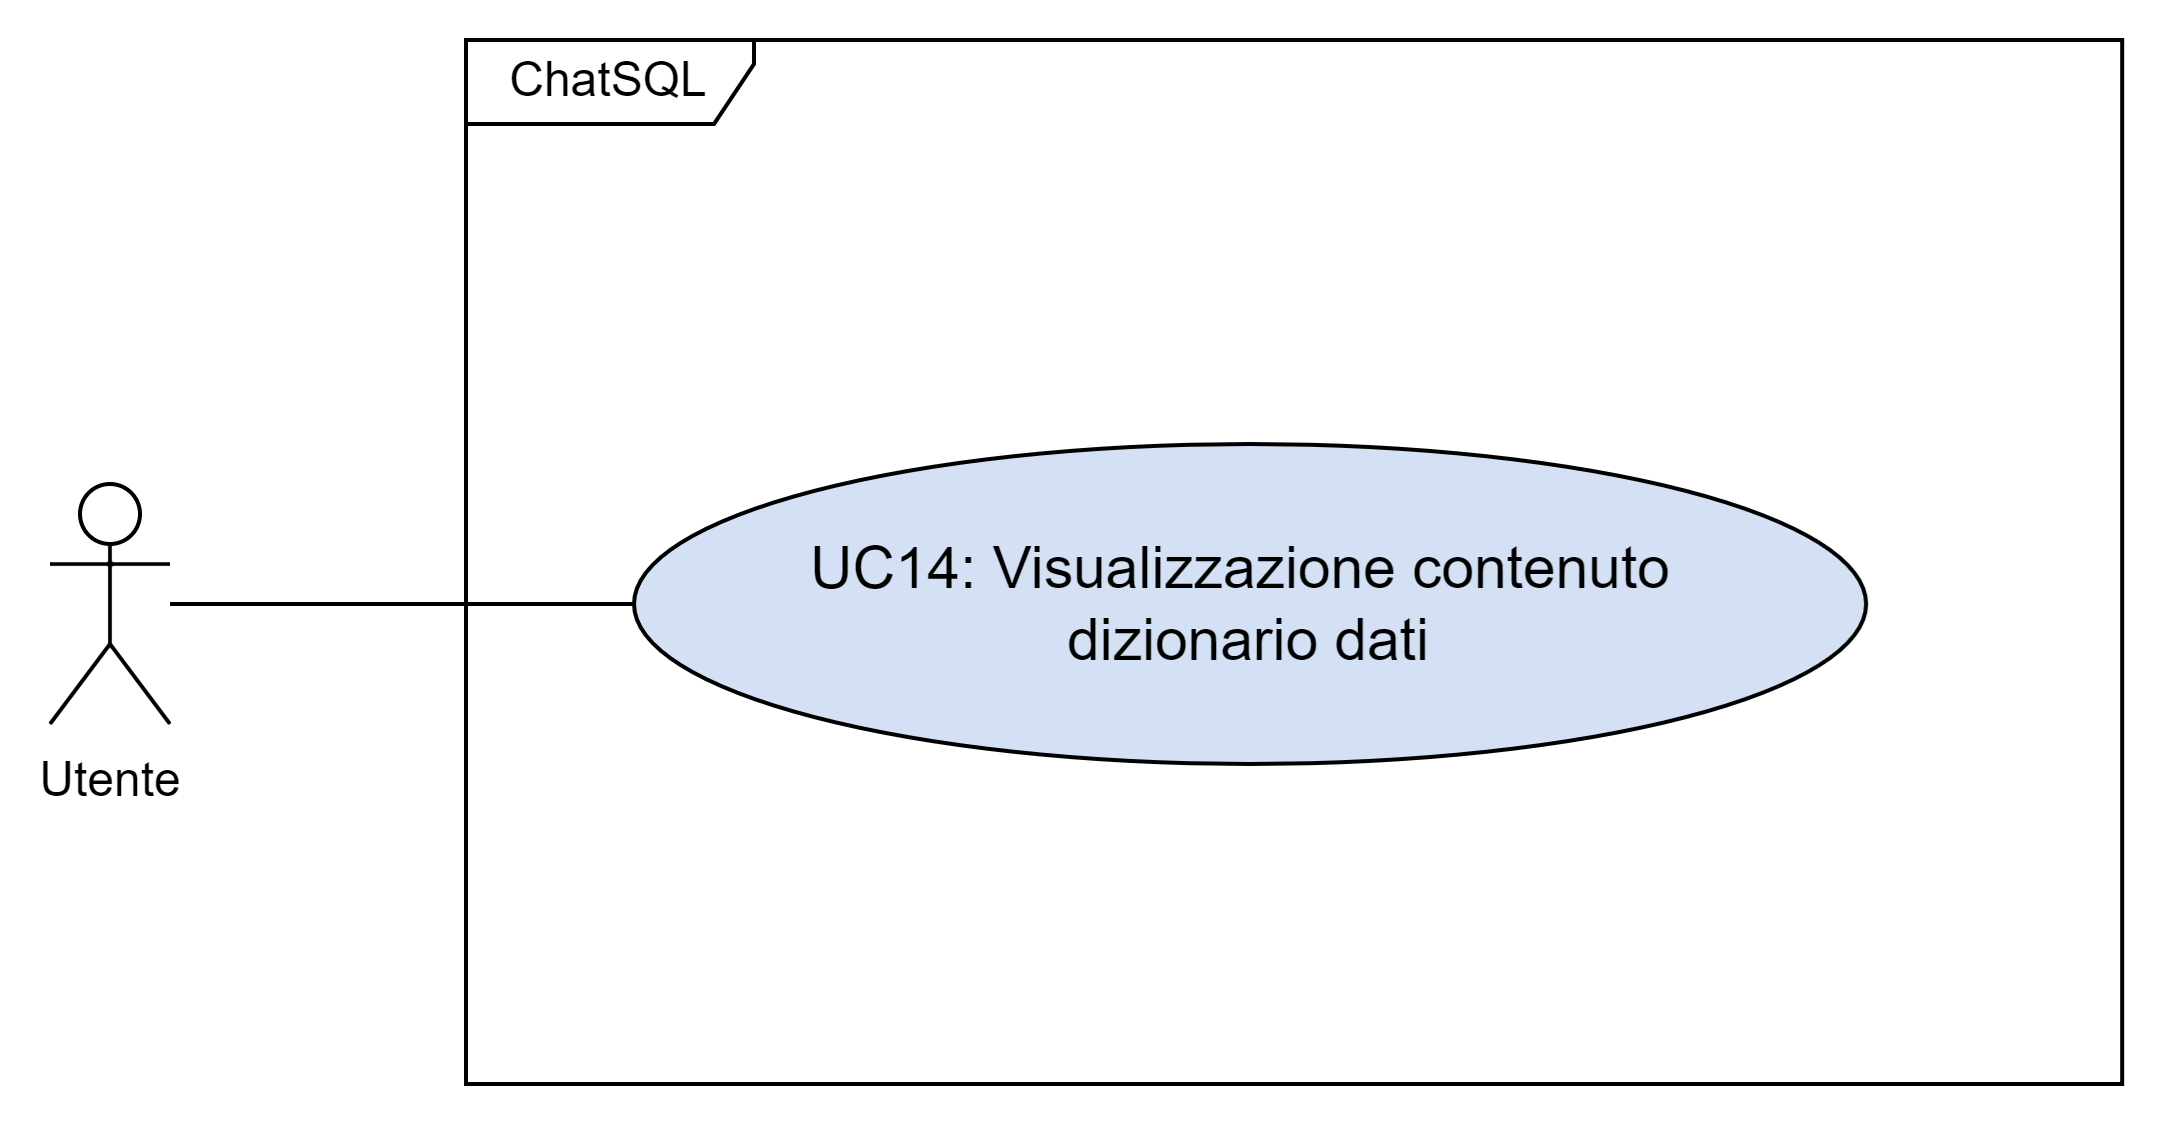
\includegraphics[width=0.90\textwidth]{assets/uc14.png}
  \caption{UC14}
\end{figure}

\paragraph*{Descrizione}
L'Utente visualizza il contenuto del \glossario{dizionario dati} selezionato. La visualizzazione del contenuto del dizionario può aiutare l'Utente a formulare correttamente la richiesta per il \glossario{modello}. Questa operazione equivale a visualizzare un'anteprima del dizionario dati.

\paragraph*{Attori principali}
Utente

\paragraph*{Precondizioni}
\begin{itemize}
  \item Il sistema è attivo e funzionante;
  \item L'Utente ha selezionato un \glossario{dizionario dati} (\hyperref[UC4]{UC4}).
\end{itemize}

\paragraph*{Postcondizioni}
\begin{itemize}
  \item Viene visualizzato il contenuto del dizionario scelto.
\end{itemize}

\paragraph*{Trigger}
L'Utente desidera visualizzare il contenuto di un \glossario{dizionario dati}.

\paragraph*{Scenario principale}
\begin{enumerate}
  \item Il sistema mostra il contenuto del dizionario in un formato comprensibile per l'Utente.
\end{enumerate}

\paragraph*{Sottocasi d'uso:}
\begin{itemize}
  \item \hyperref[UC14point1]{UC14.1}: Visualizzazione nome database;
  \item \hyperref[UC14point2]{UC14.2}: Visualizzazione descrizione database;
  \item \hyperref[UC14point3]{UC14.3}: Visualizzazione lista tabelle.
\end{itemize}

\begin{figure}[H]
  \centering
  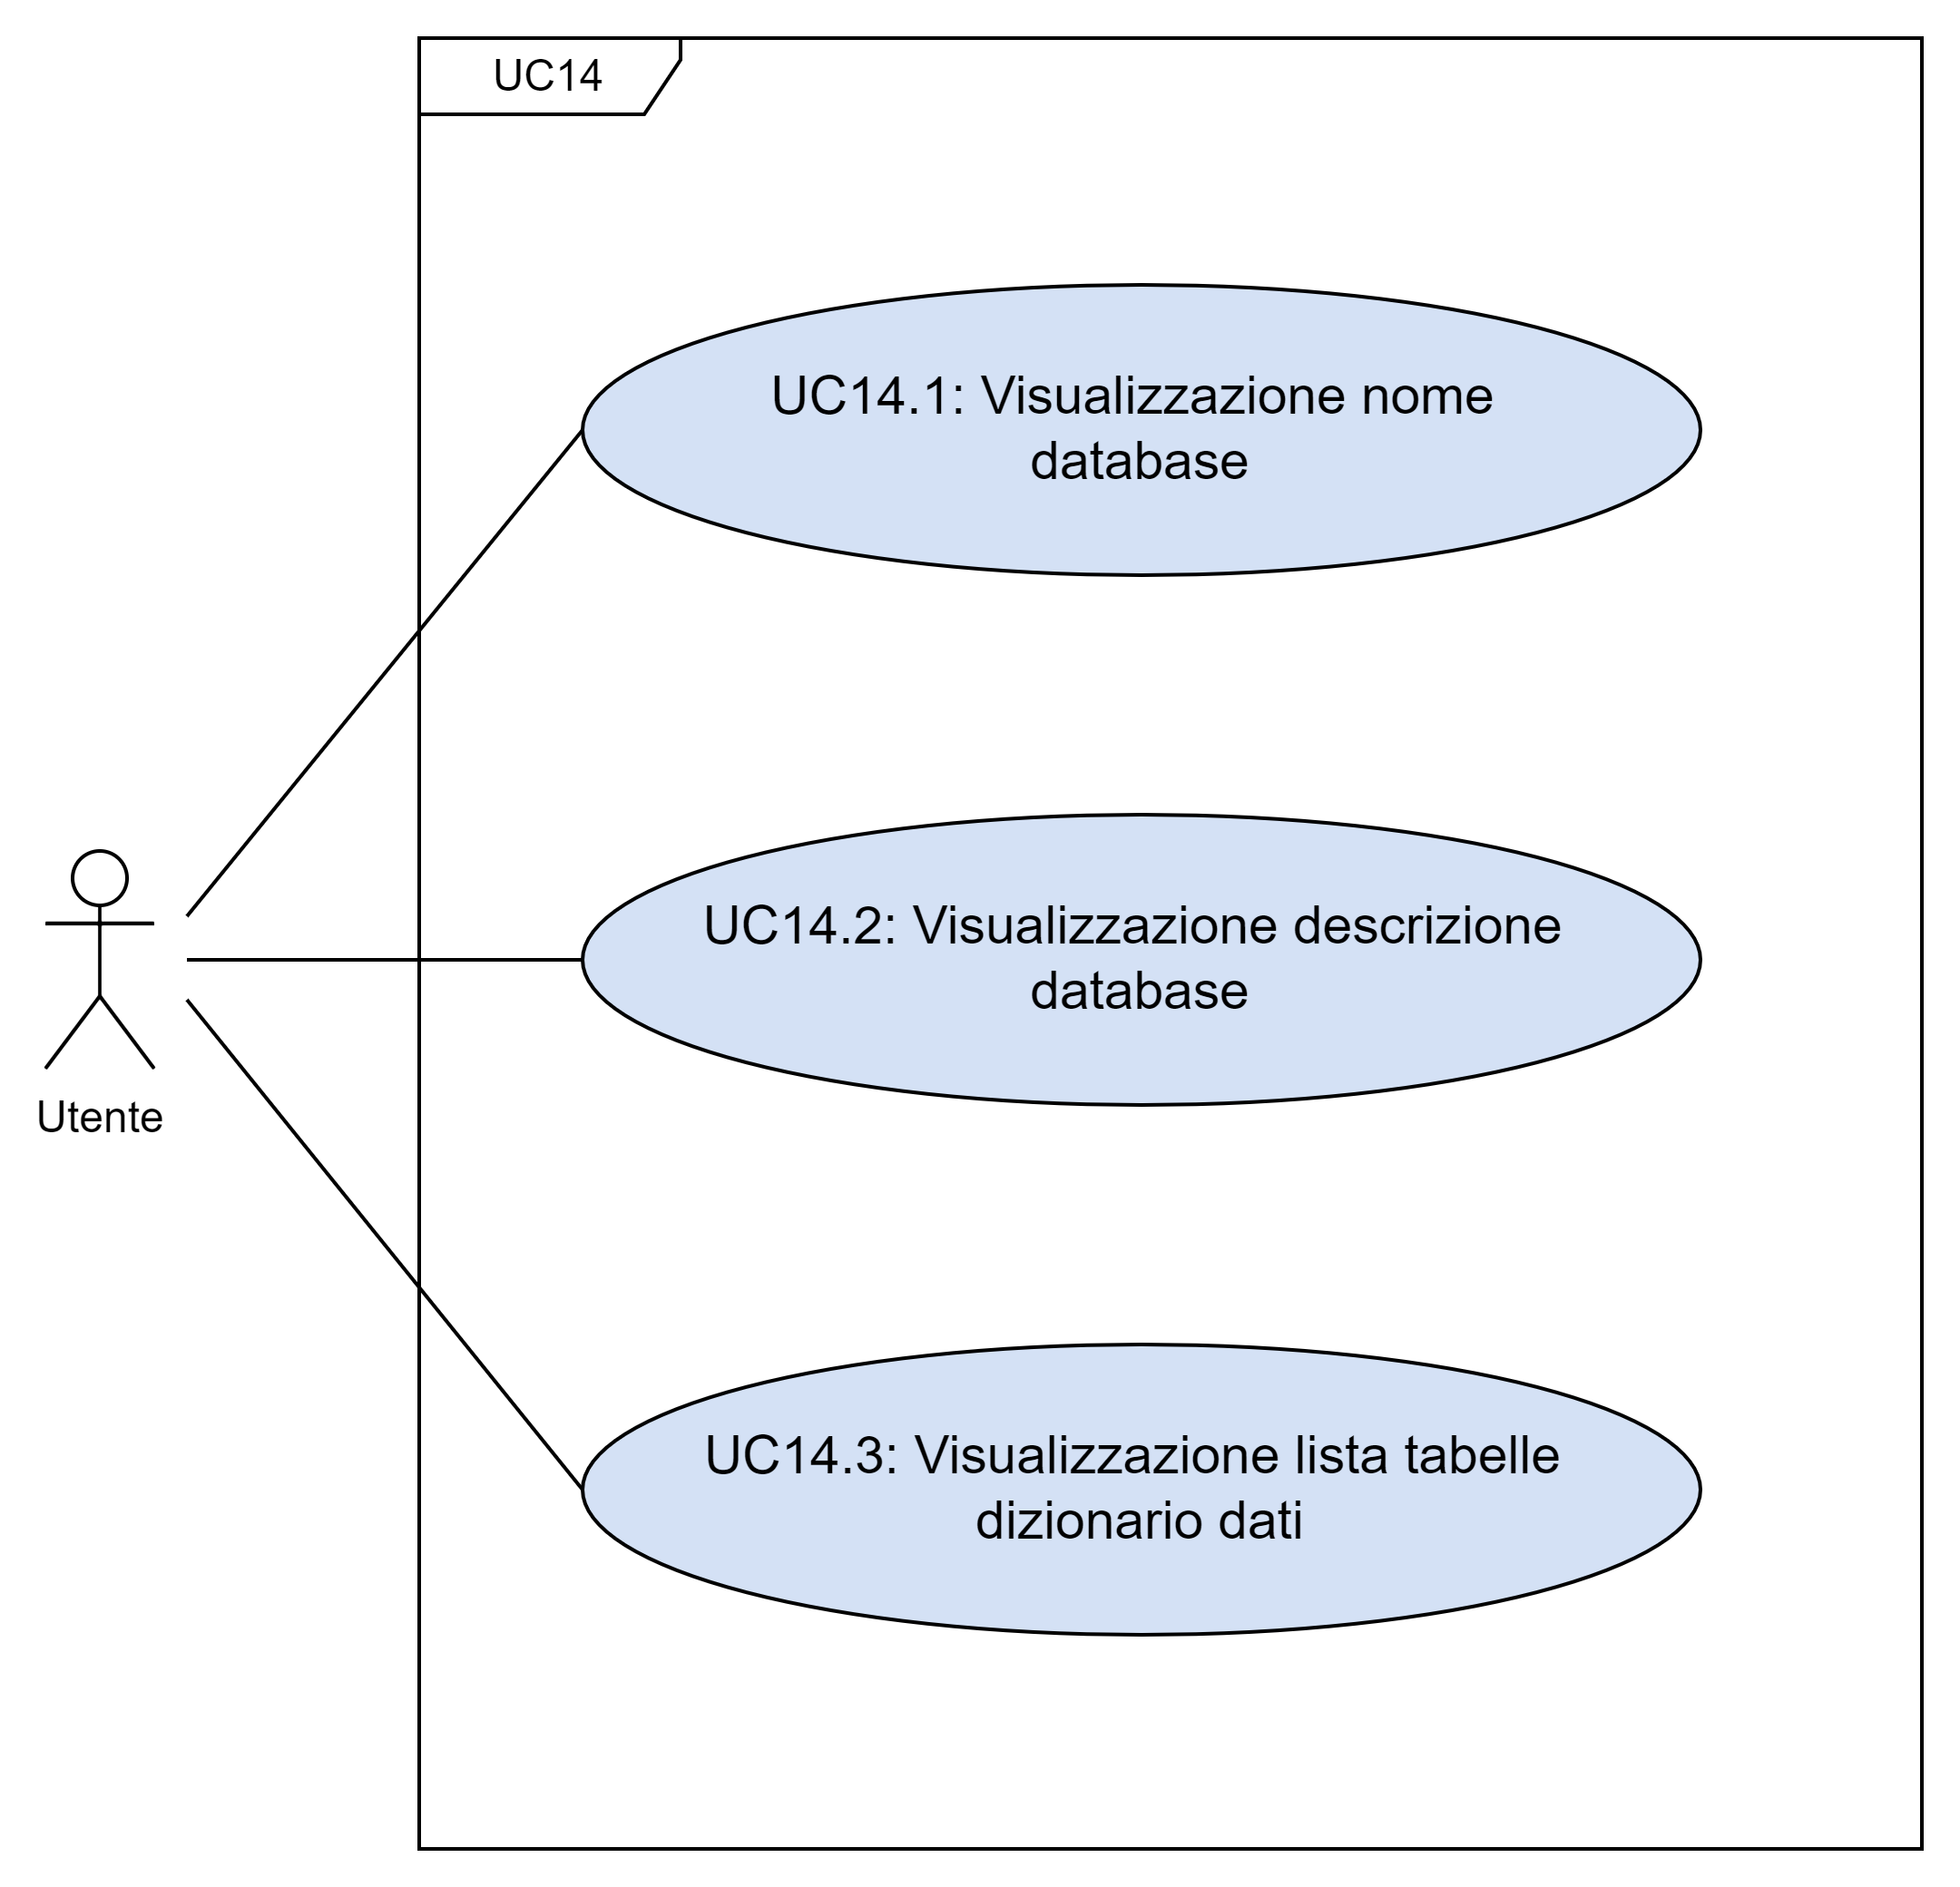
\includegraphics[width=0.90\textwidth]{assets/uc14_1.png}
  \caption{UC14 - Sottocasi d'uso}
\end{figure}

%%%%%%%%%%%%%%%%%%%%%%%%%%%%%%%%%%%%%%%%%%%%%%%%%%%%%%%%%%%%%%%%%%%%%%%%%%%%%%

\subsubsection{UC14.1 - Visualizzazione nome database}\label{UC14point1}
\paragraph*{Descrizione}
L'Utente visualizza il nome del database descritto nel \glossario{dizionario dati}.

\paragraph*{Attori principali}
Utente

\paragraph*{Precondizioni}
\begin{itemize}
  \item L'Utente ha selezionato un \glossario{dizionario dati} (\hyperref[UC4]{UC4}).
\end{itemize}

\paragraph*{Postcondizioni}
\begin{itemize}
  \item Il nome del database viene visualizzato correttamente.
\end{itemize}

\paragraph*{Trigger}
L'Utente desidera visualizzare il nome del database.

\paragraph*{Scenario principale}
\begin{enumerate}
  \item L'Utente visualizza il nome del database.
\end{enumerate}

%%%%%%%%%%%%%%%%%%%%%%%%%%%%%%%%%%%%%%%%%%%%%%%%%%%%%%%%%%%%%%%%%%%%%%%%%%%%%%

\subsubsection{UC14.2 - Visualizzazione descrizione database}\label{UC14point2}
\paragraph*{Descrizione}
L'Utente visualizza la descrizione del database riportato nel \glossario{dizionario dati}.

\paragraph*{Attori principali}
Utente

\paragraph*{Precondizioni}
\begin{itemize}
  \item L'Utente ha selezionato un \glossario{dizionario dati} (\hyperref[UC4]{UC4}).
\end{itemize}

\paragraph*{Postcondizioni}
\begin{itemize}
  \item La descrizione del database viene visualizzata correttamente.
\end{itemize}

\paragraph*{Trigger}
L'Utente desidera visualizzare la descrizione del database.

\paragraph*{Scenario principale}
\begin{enumerate}
  \item L'Utente visualizza la descrizione del database.
\end{enumerate}

%%%%%%%%%%%%%%%%%%%%%%%%%%%%%%%%%%%%%%%%%%%%%%%%%%%%%%%%%%%%%%%%%%%%%%%%%%%%%%

\subsubsection{UC14.3 - Visualizzazione lista tabelle dizionario dati}\label{UC14point3}
\paragraph*{Descrizione}
L'Utente visualizza la lista delle tabelle descritte nel \glossario{dizionario dati}.

\paragraph*{Attori principali}
Utente

\paragraph*{Precondizioni}
\begin{itemize}
  \item L'Utente ha selezionato un \glossario{dizionario dati} (\hyperref[UC4]{UC4}).
\end{itemize}

\paragraph*{Postcondizioni}
\begin{itemize}
  \item La lista delle tabelle viene visualizzata correttamente.
\end{itemize}

\paragraph*{Trigger}
L'Utente desidera visualizzare la lista delle tabelle.

\paragraph*{Scenario principale}
\begin{enumerate}
  \item L'Utente visualizza la lista delle tabelle.
\end{enumerate}

\paragraph*{Sottocasi d'uso:}
\begin{itemize}
  \item \hyperref[UC14point3point1]{UC14.3.1}: Visualizzazione singola tabella.
\end{itemize}

%%%%%%%%%%%%%%%%%%%%%%%%%%%%%%%%%%%%%%%%%%%%%%%%%%%%%%%%%%%%%%%%%%%%%%%%%%%%%%

\subsubsection{UC14.3.1 - Visualizzazione singola tabella dizionario dati}\label{UC14point3point1}

\begin{figure}[H]
  \centering
  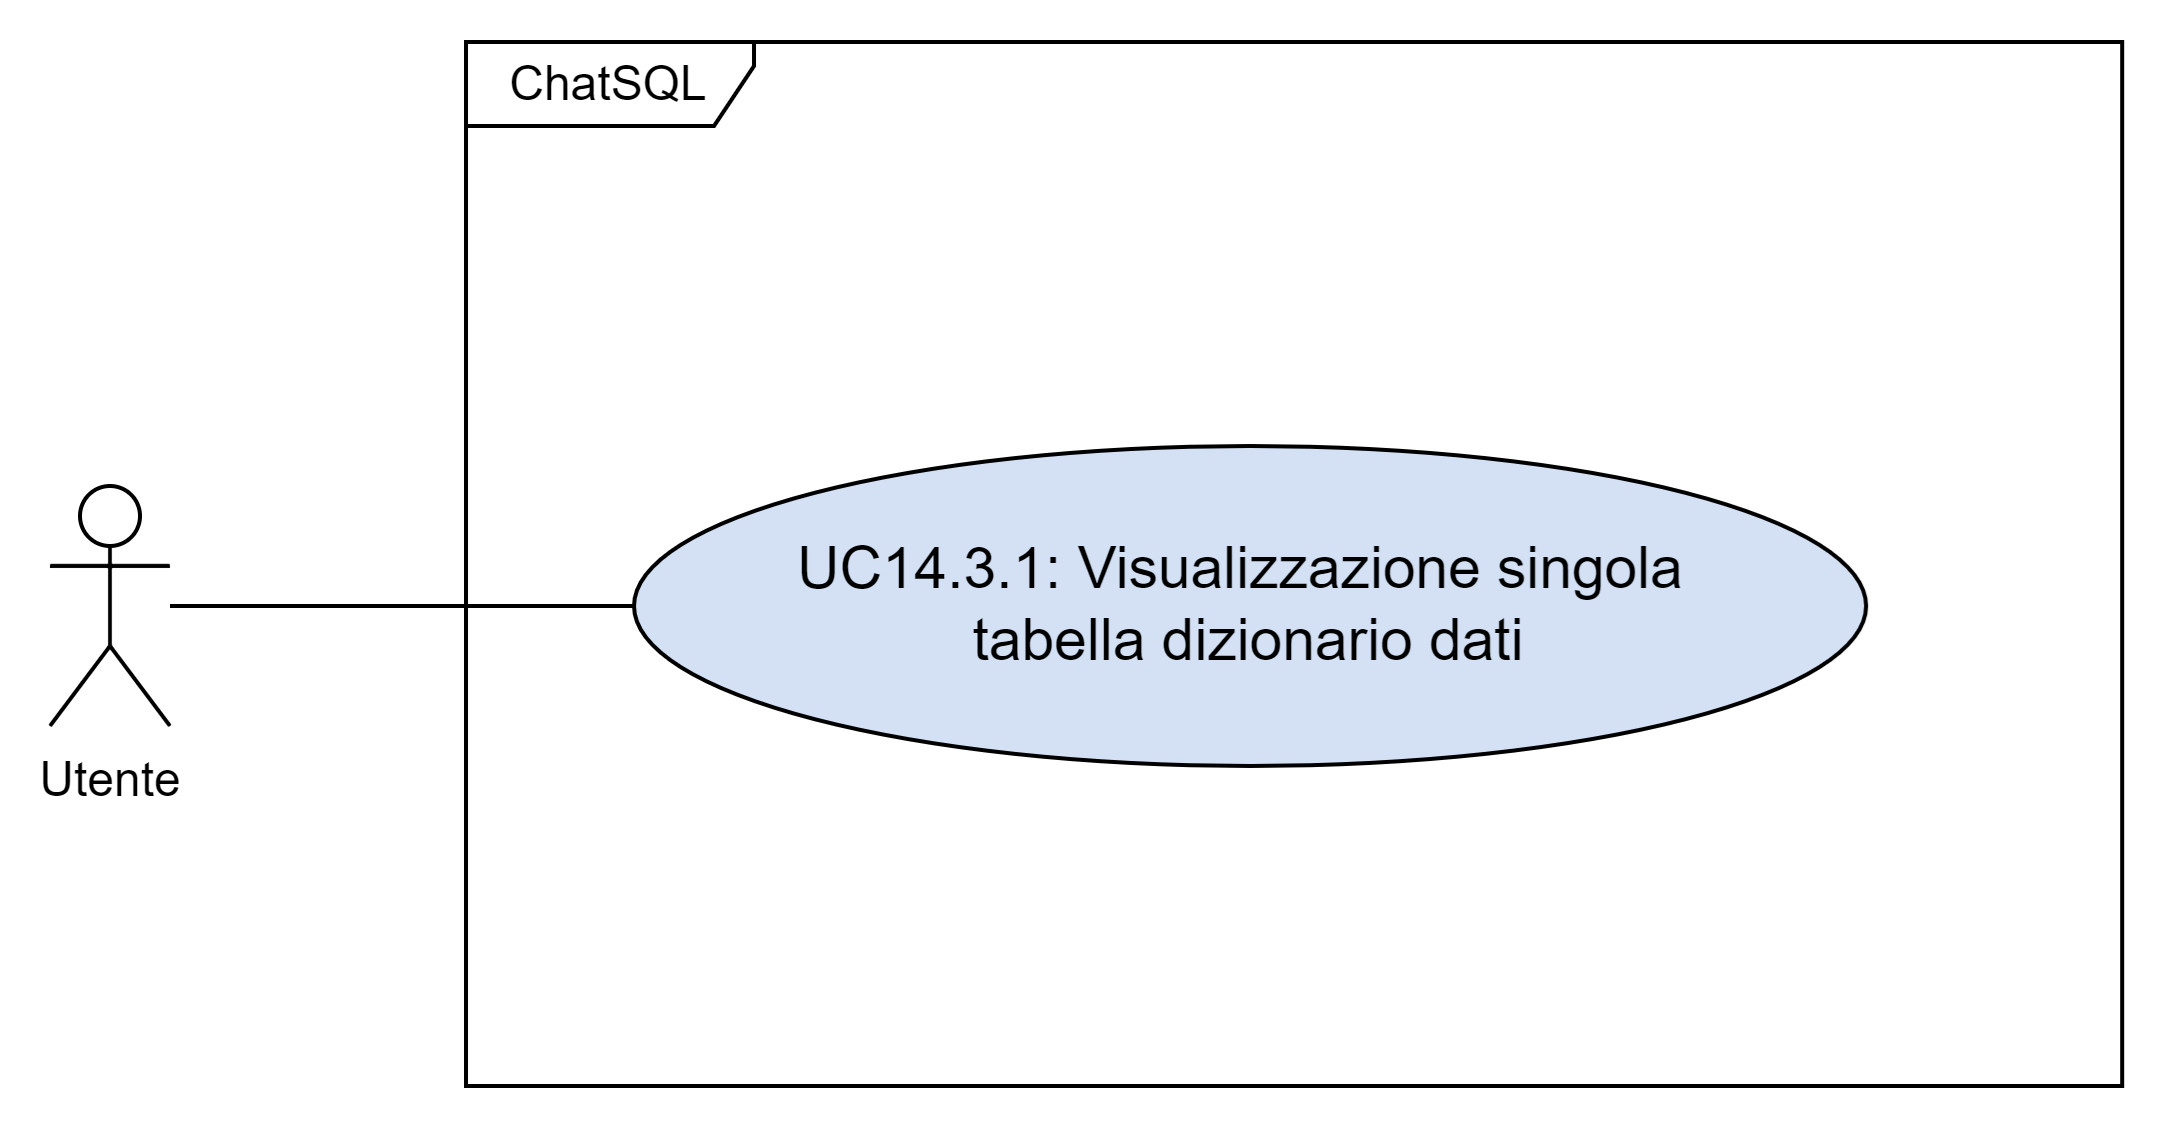
\includegraphics[width=0.90\textwidth]{assets/uc14_3_1.png}
  \caption{UC14.3.1}
\end{figure}

\paragraph*{Descrizione}
L'Utente visualizza una tabella tra quelle descritte nel \glossario{dizionario dati}.

\paragraph*{Attori principali}
Utente

\paragraph*{Precondizioni}
\begin{itemize}
  \item L'Utente ha selezionato un \glossario{dizionario dati} (\hyperref[UC4]{UC4});
  \item L'Utente ha visualizzato la lista delle tabelle (\hyperref[UC14point3]{UC14.3}).
\end{itemize}

\paragraph*{Postcondizioni}
\begin{itemize}
  \item La tabella viene visualizzata correttamente.
\end{itemize}

\paragraph*{Trigger}
L'Utente desidera visualizzare una tabella con le sue informazioni.

\paragraph*{Scenario principale}
\begin{enumerate}
  \item L'Utente visualizza una singola tabella in lista.
\end{enumerate}

\paragraph*{Sottocasi d'uso:}
\begin{itemize}
  \item \hyperref[UC14point3point1point1]{UC14.3.1.1}: Visualizzazione nome tabella;
  \item \hyperref[UC14point3point1point2]{UC14.3.1.2}: Visualizzazione descrizione tabella.
\end{itemize}

\begin{figure}[H]
  \centering
  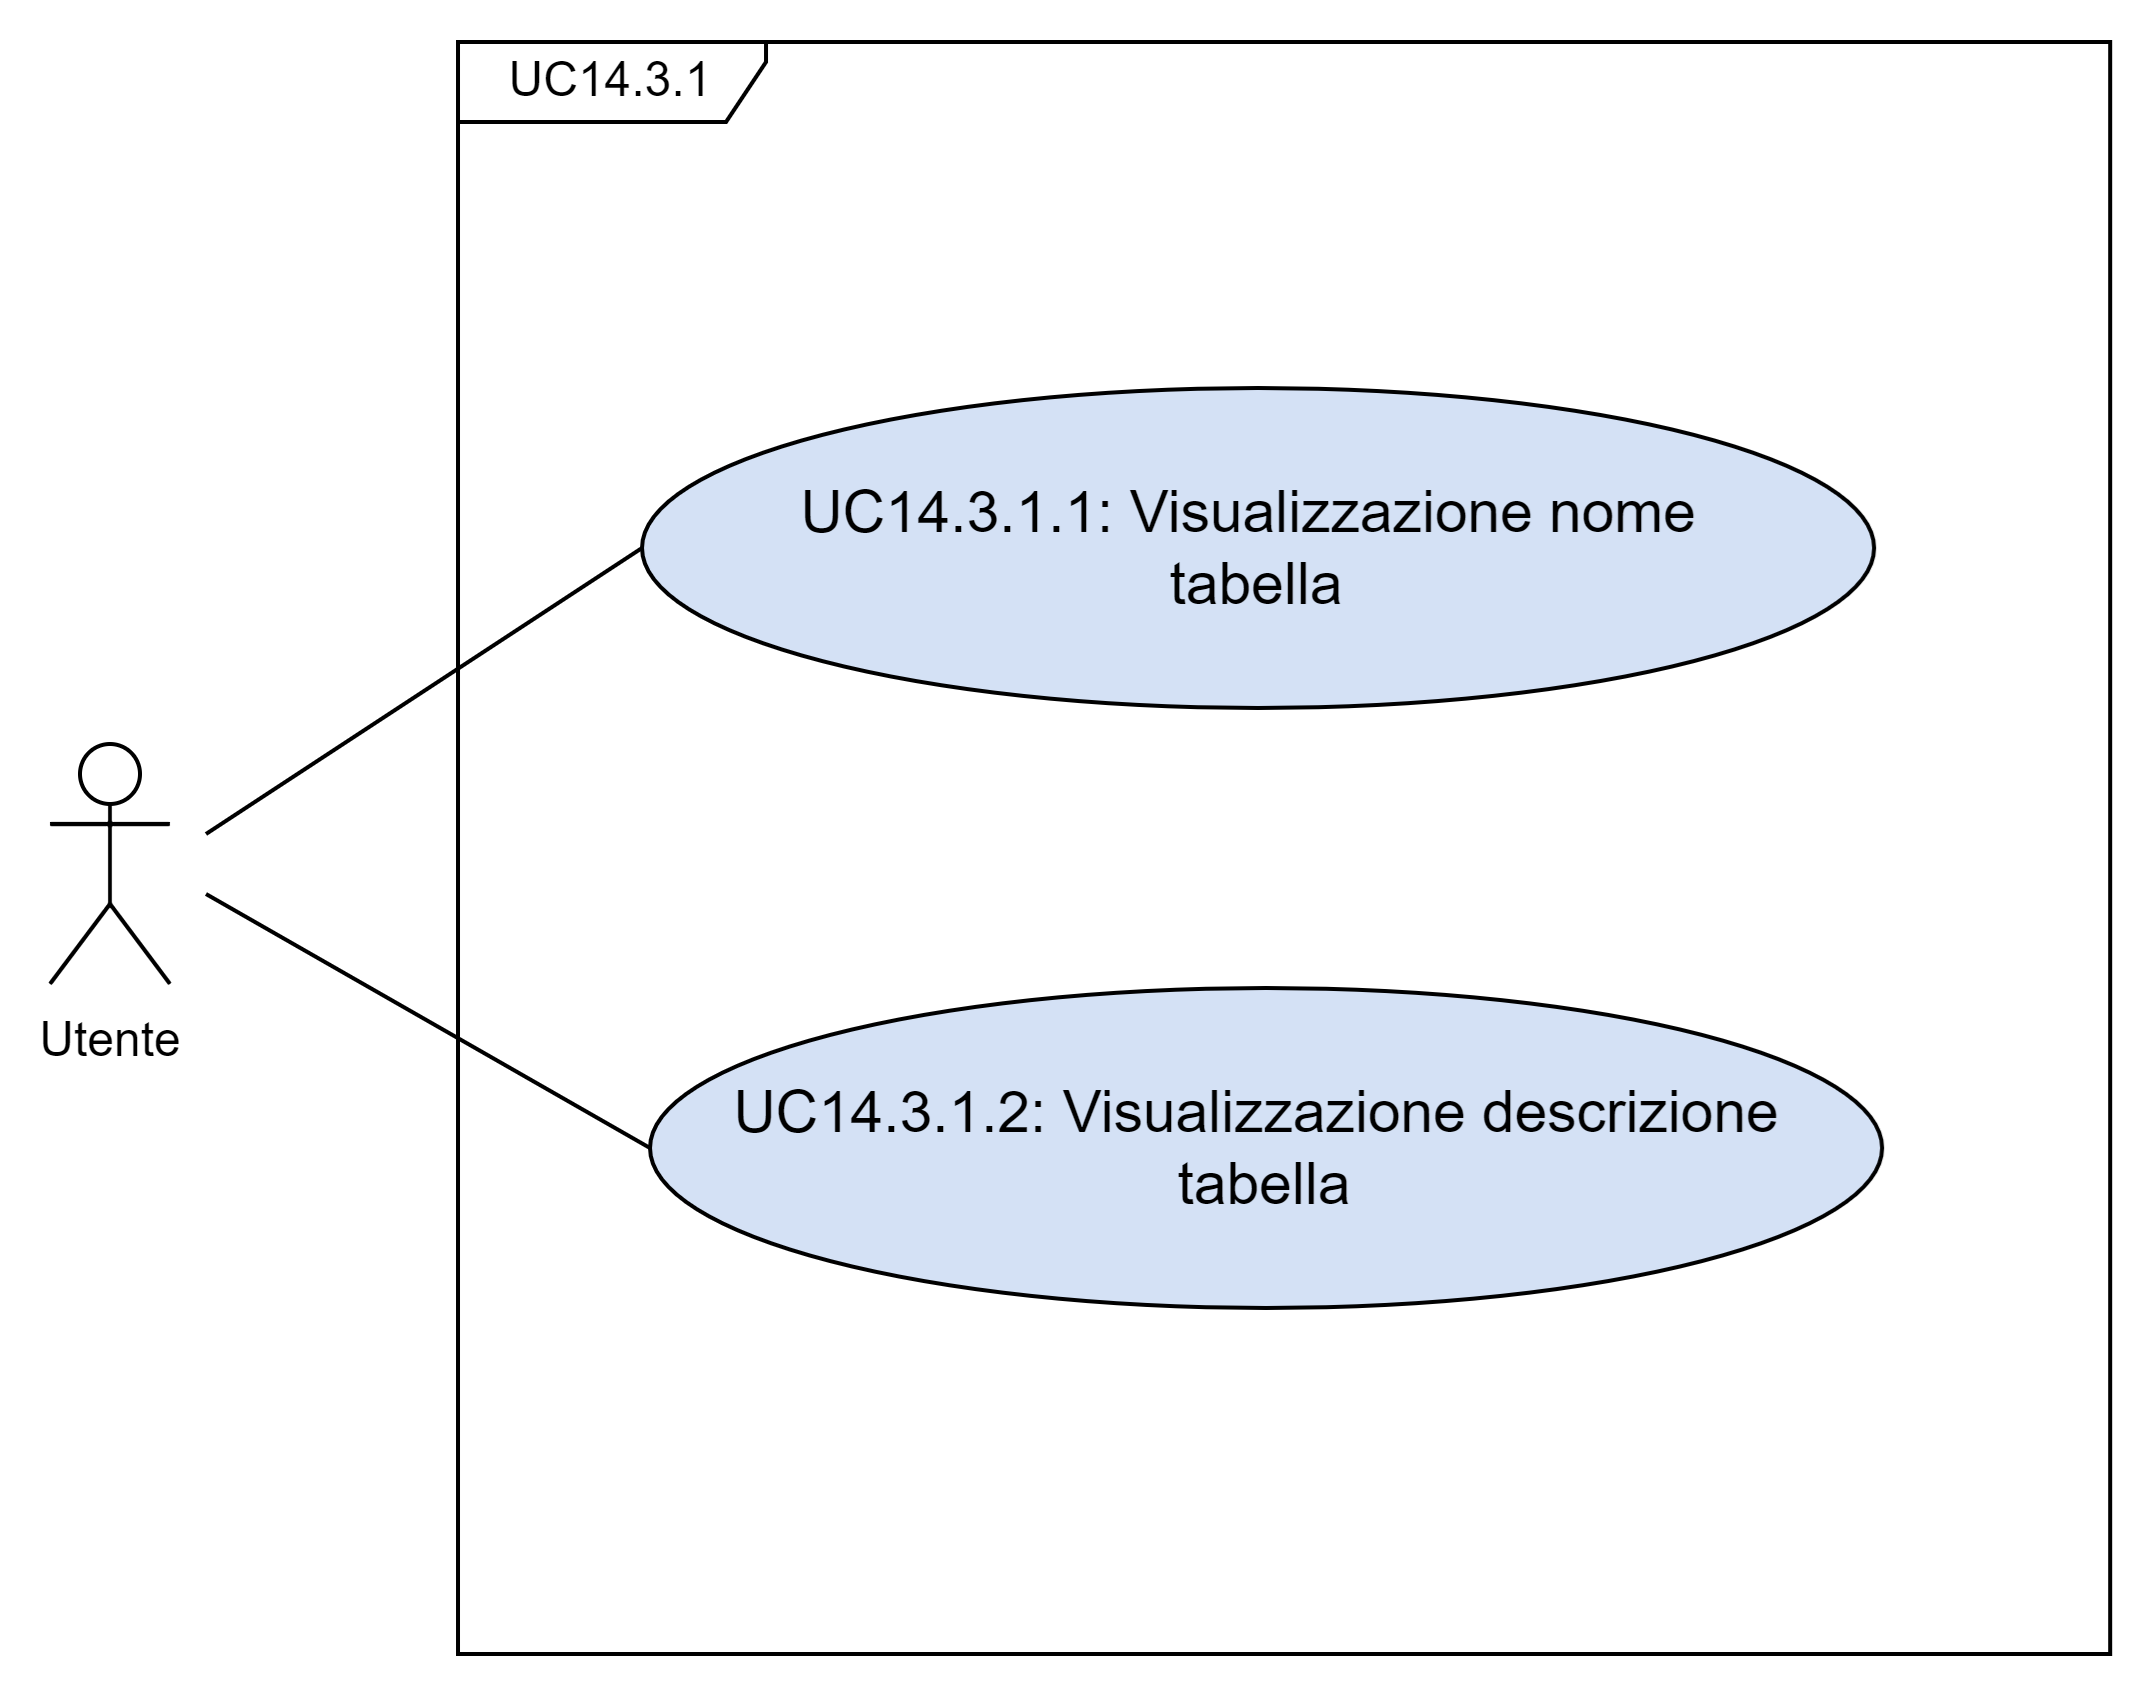
\includegraphics[width=0.90\textwidth]{assets/uc14_3_1_1.png}
  \caption{UC14.3.1 - Sottocasi d'uso}
\end{figure}

%%%%%%%%%%%%%%%%%%%%%%%%%%%%%%%%%%%%%%%%%%%%%%%%%%%%%%%%%%%%%%%%%%%%%%%%%%%%%%

\subsubsection{UC14.3.1.1 - Visualizzazione nome tabella}\label{UC14point3point1point1}
\paragraph*{Descrizione}
L'Utente visualizza il nome di una tabella.

\paragraph*{Attori principali}
Utente

\paragraph*{Precondizioni}
\begin{itemize}
  \item L'Utente ha selezionato un \glossario{dizionario dati} (\hyperref[UC4]{UC4});
  \item L'Utente ha visualizzato la lista delle tabelle (\hyperref[UC14point3]{UC14.3});
  \item L'Utente ha visualizzato una singola tabella in lista (\hyperref[UC14point3point1]{UC14.3.1}).
\end{itemize}

\paragraph*{Postcondizioni}
\begin{itemize}
  \item Il nome della tabella viene visualizzato correttamente.
\end{itemize}

\paragraph*{Trigger}
L'Utente desidera visualizzare il nome di una tabella.

\paragraph*{Scenario principale}
\begin{enumerate}
  \item L'Utente visualizza il nome di una tabella.
\end{enumerate}

%%%%%%%%%%%%%%%%%%%%%%%%%%%%%%%%%%%%%%%%%%%%%%%%%%%%%%%%%%%%%%%%%%%%%%%%%%%%%%

\subsubsection{UC14.3.1.2 - Visualizzazione descrizione tabella}\label{UC14point3point1point2}
\paragraph*{Descrizione}
L'Utente visualizza la descrizione di una tabella.

\paragraph*{Attori principali}
Utente

\paragraph*{Precondizioni}
\begin{itemize}
  \item L'Utente ha selezionato un \glossario{dizionario dati} (\hyperref[UC4]{UC4});
  \item L'Utente ha visualizzato la lista delle tabelle (\hyperref[UC14point3]{UC14.3});
  \item L'Utente ha visualizzato una singola tabella in lista (\hyperref[UC14point3point1]{UC14.3.1}).
\end{itemize}

\paragraph*{Postcondizioni}
\begin{itemize}
  \item La descrizione della tabella viene visualizzata correttamente.
\end{itemize}

\paragraph*{Trigger}
L'Utente desidera visualizzare la descrizione di una tabella.

\paragraph*{Scenario principale}
\begin{enumerate}
  \item L'Utente visualizza la descrizione di una tabella.
\end{enumerate}
\subsubsection{UC15 - Caricamento file dizionario dati}\label{UC15}

\paragraph*{Descrizione}
L'Utene carica un \glossario{dizionario dati} da salvare nel sistema.

\paragraph*{Attori principali}
Tecnico

\paragraph*{Precondizioni}
\begin{itemize}
  \item Il sistema è attivo e funzionante;
  \item Il Tecnico ha effettuato correttamente l'autenticazione (\hyperref[UC1]{UC1}).
\end{itemize}

\paragraph*{Postcondizioni}
\begin{itemize}
  \item Il \glossario{dizionario dati} è stato caricato correttamente.
\end{itemize}

\paragraph*{Trigger}
Il Tecnico vuole caricare un \glossario{dizionario dati} da utilizzare per la generazione di \glossario{prompt}.

\paragraph*{Scenario principale}
\begin{enumerate}
  \item Il Tecnico avvia la procedura di caricamento di un nuovo \glossario{dizionario dati};
  \item Il sistema permette al Tecnico di inserire un file nel formato appropriato;
  \item Il Tecnico inserisce il file;
  \item Vengono visualizzati il nome e l'estensione del file caricato.
\end{enumerate}

\subsubsection{UC16 - Inserimento nome dizionario dati}\label{UC16}
\paragraph*{Descrizione}
Il Tecnico inserisce il nome di un \glossario{dizionario dati}.

\paragraph*{Attori principali}
Tecnico

\paragraph*{Precondizioni}
\begin{itemize}
  \item Il sistema è attivo e funzionante;
  \item Il Tecnico ha effettuato l'autenticazione (\hyperref[UC1]{UC1}).
\end{itemize}

\paragraph*{Postcondizioni}
\begin{itemize}
  \item Il nome del \glossario{dizionario dati} è stato inserito correttamente.
\end{itemize}

\paragraph*{Trigger}
Il Tecnico vuole inserire il nome di un \glossario{dizionario dati}.

\paragraph*{Scenario principale}
\begin{enumerate}
  \item Il Tecnico scrive il nome del \glossario{dizionario dati} nell'apposito campo di testo.
\end{enumerate}
\subsubsection{UC17 - Inserimento descrizione dizionario dati}\label{UC17}
\paragraph*{Descrizione}
Il Tecnico inserisce la descrizione di un \glossario{dizionario dati}.

\paragraph*{Attori principali}
Tecnico

\paragraph*{Precondizioni}
\begin{itemize}
  \item Il sistema è attivo e funzionante;
  \item Il Tecnico ha effettuato l'autenticazione (\hyperref[UC1]{UC1}).
\end{itemize}

\paragraph*{Postcondizioni}
\begin{itemize}
  \item La descrizione del \glossario{dizionario dati} è stata inserita correttamente.
\end{itemize}

\paragraph*{Trigger}
Il Tecnico vuole inserire la descrizione di un \glossario{dizionario dati}.

\paragraph*{Scenario principale}
\begin{enumerate}
  \item Il Tecnico scrive la descrizione del \glossario{dizionario dati} nell'apposito campo di testo.
\end{enumerate}
\subsubsection{UC18 - Debug della generazione del \glossario{prompt}}\label{UC18}

\paragraph*{Descrizione}
Il Tecnico vuole poter testare il \glossario{prompt} generato e interroga il sistema per comprendere la corretta formattazione del \glossario{dizionario dati}. Visualizza una tabella contenente i campi del \glossario{dizionario dati} e lo score ottenuto per questi.

\paragraph*{Attori principali}
Tecnico

\paragraph*{Precondizioni}
\begin{itemize}
  \item Il Tecnico è correttamente autenticato tramite login (\hyperref[UC1]{UC1});
  \item È presente almeno un \glossario{dizionario dati} nel sistema;
  \item Il Tecnico inserisce una richiesta in linguaggio naturale (\hyperref[UC3]{UC3});
  \item Il sistema genera il \glossario{prompt} (\hyperref[UC5]{UC5});
  \item Il Tecnico seleziona lo strumento di debug.
\end{itemize}

\paragraph*{Postcondizioni}
\begin{itemize}
  \item Il sistema genera un \glossario{log};
  \item Il sistema genera una tabella dei migliori risultati individuati;
\end{itemize}

\paragraph*{Scenario principale}
\begin{enumerate}
  \item Il Tecnico riceve il \glossario{prompt} dal sistema (\hyperref[UC5]{UC5});
  \item Il Tecnico seleziona lo strumento di debug;
  \item Lo strumento di debug genera una tabella dei risultati individuati dal sistema; 
  \item Lo strumento di debug genera un \glossario{log} descrittivo dei passaggi per la composizione del \glossario{prompt}.  
\end{enumerate}

\paragraph*{Inclusione}
\begin{itemize}
  \item Visualizzazione della singola riga della tabella. %UC18.1
\end{itemize}

\paragraph*{Estensione}
\begin{itemize}
  \item Messaggio d'errore nella generazione del \glossario{prompt} (\hyperref[UC6]{UC6}).
  \item Download del \glossario{log}. %UC19
\end{itemize}

\subsubsection{UC19 - Visualizzazione errore validazione file}\label{UC19}

\begin{figure}[H]
  \centering
  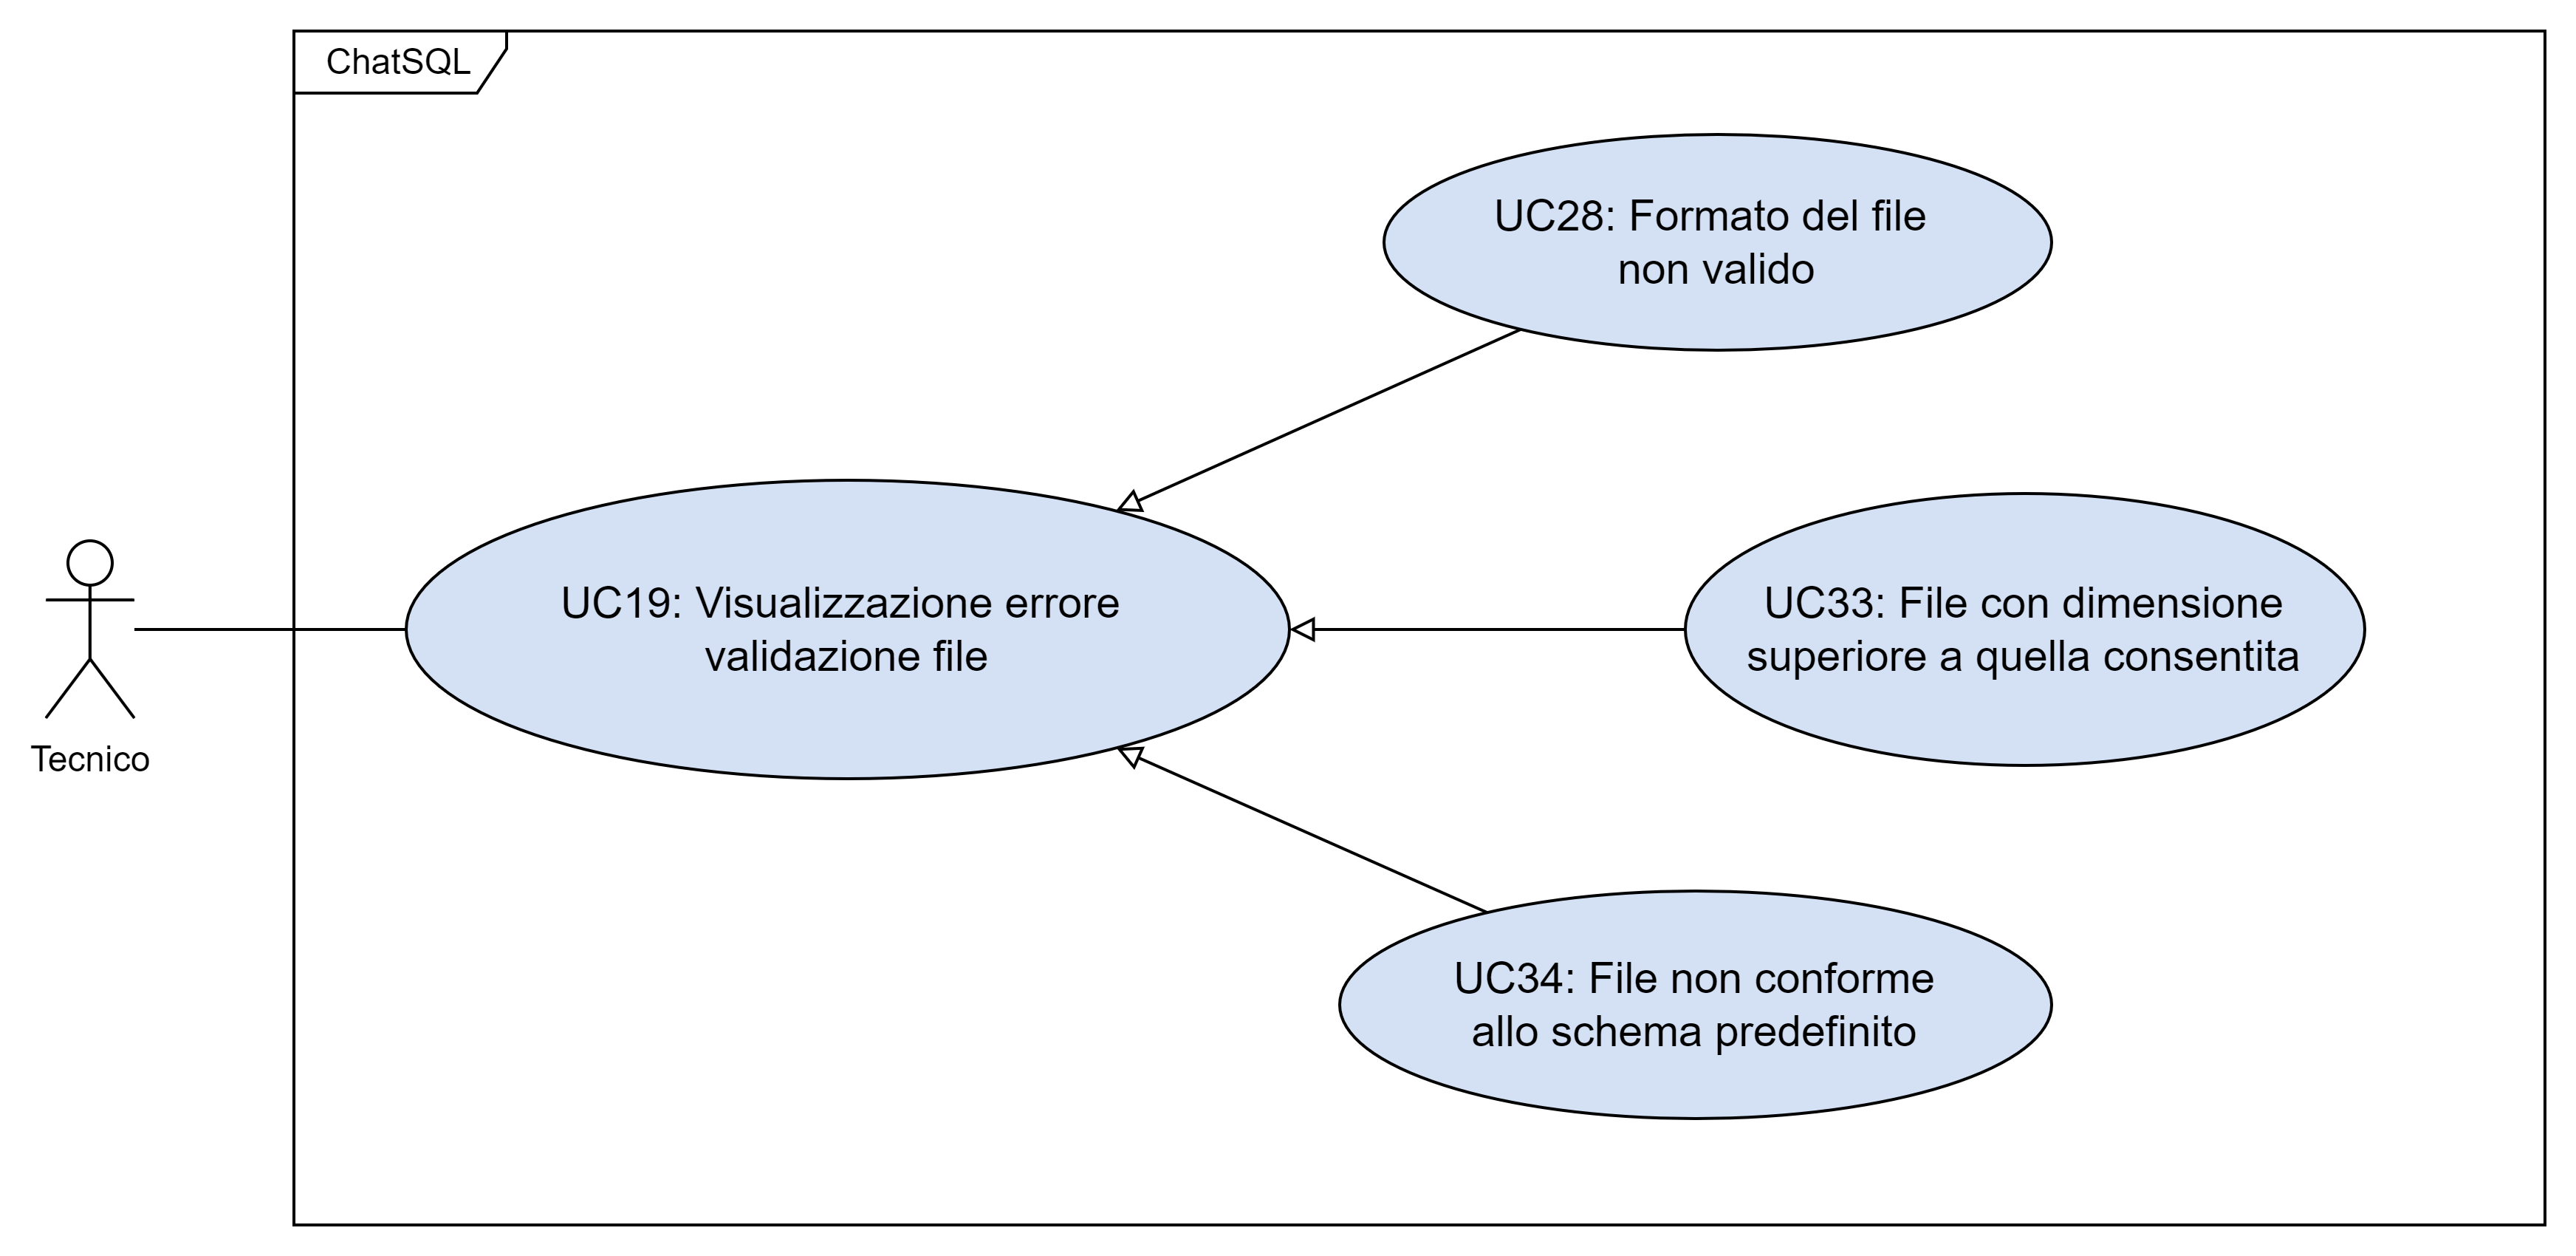
\includegraphics[width=0.90\textwidth]{assets/uc19.png}
  \caption{UC19}
\end{figure}

\paragraph*{Descrizione}
Nel caso in cui il sistema riscontri delle anomalie nella validazione del file scelto come \glossario{dizionario dati}, il Tecnico visualizza un messaggio d'errore.

\paragraph*{Attori principali}
Tecnico

\paragraph*{Precondizioni}
\begin{itemize}
  \item Il Tecnico ha richiesto il salvataggio o la modifica di un \glossario{dizionario dati} nel sistema;
  \item Il file caricato non è valido.
\end{itemize}

\paragraph*{Postcondizioni}
\begin{itemize}
  \item Viene mostrato un messaggio d'errore esplicativo;
  \item L'operazione di salvataggio o modifica non viene portata a termine.
\end{itemize}

\paragraph*{Scenario principale}
\begin{enumerate}
  \item Il sistema riscontra un errore nella validazione del file scelto come \glossario{dizionario dati};
  \item Il sistema restituisce un messaggio con i dettagli dell'errore. 
\end{enumerate}

\paragraph*{Specializzazioni}
\begin{itemize}
  \item Formato del file non valido (\hyperref[UC28]{UC28});
  \item File troppo pesante (\hyperref[UC33]{UC33});
  \item File non conforme allo schema predefinito (\hyperref[UC34]{UC34}).
\end{itemize}
\subsubsection{UC20 - Errore per modifica incorretta del \glossario{dizionario dati}}\label{UC20}
\paragraph*{Descrizione}
Il sistema mostra un messaggio d’errore relativo ad una modifica incorretta del \glossario{dizionario dati}.

\paragraph*{Attori principali}
Tecnico

\paragraph*{Precondizioni}
\begin{itemize}
  \item Il Tecnico è correttamente autenticato tramite login (\hyperref[UC1]{UC1});
  \item Il Tecnico ha visualizza i dettagli del \glossario{dizionario dati} da modificare (\hyperref[UC14]{UC14});
  \item Il Tecnico sceglie di modificare il \glossario{dizionario dati} individuato (\hyperref[UC16]{UC16}).
\end{itemize}

\paragraph*{Postcondizioni}
\begin{itemize}
  \item Il sistema mostra un messaggio d’errore dovuto ad una modifica invalida.
\end{itemize}

\paragraph*{Scenario principale}
\begin{enumerate}
  \item Il Tecnico ha avviato la procedura di modifica del \glossario{dizionario dati} (\hyperref[UC16]{UC16});
  \item Il Tecnico modifica il \glossario{dizionario dati};
  \item Il sistema riscontra un errore nella modifica;
  \item Viene mostrato un messaggio d'errore con il dettaglio dell'invalidità nella modifica.  
\end{enumerate}

\paragraph*{Inclusioni}
\begin{itemize}
    \item Errore per modifica incorretta del titolo del \glossario{dizionario dati} (\hyperref[UC20point1]{UC20.1});
    \item Errore per modifica incorretta della descrizione del \glossario{dizionario dati} (\hyperref[UC20point2]{UC20.2});
    \item Errore per mancato caricamento del \glossario{dizionario dati} (\hyperref[UC19]{UC19}).
\end{itemize}

%%%%%%%%%%%%%%%%%%%%%%%%%%%%%%%%%%%%%%%%%%%%%%%%%%%

\subsubsection{UC20.1 - Errore per modifica incorretta del titolo del \glossario{dizionario dati}}\label{UC20point1}
\paragraph*{Descrizione}
Il sistema mostra un messaggio d’errore relativo ad una modifica del titolo con un formato invalido.

\paragraph*{Attori principali}
Tecnico

\paragraph*{Precondizioni}
\begin{itemize}
  \item Il Tecnico è correttamente autenticato tramite login (\hyperref[UC1]{UC1});
  \item Il Tecnico sceglie di modificare il \glossario{dizionario dati} individuato (\hyperref[UC16]{UC16});
  \item Il Tecnico sceglie di modificare il titolo.
\end{itemize}

\paragraph*{Postcondizioni}
\begin{itemize}
  \item Il sistema mostra un messaggio d’errore dovuto ad una modifica con formato invalido del titolo.
\end{itemize}

\paragraph*{Scenario principale}
\begin{enumerate}
  \item Il Tecnico ha avviato la procedura di modifica del \glossario{dizionario dati} (\hyperref[UC16]{UC16});
  \item Il Tecnico modifica il titolo del \glossario{dizionario dati};
  \item Il sistema riscontra un errore nella modifica del titolo;
  \item Viene mostrato un messaggio d'errore con il dettaglio dell'invalidità nella modifica.  
\end{enumerate}

%%%%%%%%%%%%%%%%%%%%%%%%%%%%%%%%%%%%%%%%%%%%%%%%

\subsubsection{UC20.2 - Errore per modifica incorretta della descrizione del \glossario{dizionario dati}}\label{UC20point2}
\paragraph*{Descrizione}
Il sistema mostra un messaggio d’errore relativo ad una modifica della descrizione con un formato invalido.

\paragraph*{Attori principali}
Tecnico

\paragraph*{Precondizioni}
\begin{itemize}
  \item Il Tecnico è correttamente autenticato tramite login (\hyperref[UC1]{UC1});
  \item Il Tecnico sceglie di modificare il \glossario{dizionario dati} individuato (\hyperref[UC16]{UC16});
  \item Il Tecnico sceglie di modificare la descrizione.
\end{itemize}

\paragraph*{Postcondizioni}
\begin{itemize}
  \item Il sistema mostra un messaggio d’errore dovuto ad una modifica con formato invalido della descrizione.
\end{itemize}

\paragraph*{Scenario principale}
\begin{enumerate}
  \item Il Tecnico ha avviato la procedura di modifica del \glossario{dizionario dati} (\hyperref[UC16]{UC16});
  \item Il Tecnico modifica la descrizione del \glossario{dizionario dati};
  \item Il sistema riscontra un errore nella modifica della descrizione;
  \item Viene mostrato un messaggio d'errore con il dettaglio dell'invalidità nella modifica.  
\end{enumerate}
\subsubsection{UC21 - Visualizzazione errore eliminazione dizionario dati}\label{UC21}
\paragraph*{Descrizione}
Il sistema mostra un messaggio di errore a causa della mancata eliminazione di un \glossario{dizionario dati}.

\paragraph*{Attori principali}
Tecnico

\paragraph*{Precondizioni}
\begin{itemize}
  \item Il Tecnico ha effettuato l'autenticazione (\hyperref[UC1]{UC1});
  \item Il Tecnico ha richiesto l'eliminazione di un \glossario{dizionario dati} (\hyperref[UC18]{UC18});
  \item Il sistema ha riscontrato un errore nel tentativo di eliminare il dizionario dati.
\end{itemize}

\paragraph*{Postcondizioni}
\begin{itemize}
  \item Viene visualizzato un messaggio d'errore esplicativo;
  \item Il \glossario{dizionario dati} non viene rimosso dal sistema.
\end{itemize}

\paragraph*{Scenario principale}
\begin{enumerate}
  \item Il sistema restituisce un messaggio con i dettagli dell'errore.
\end{enumerate}
\subsubsection{UC25 - Visualizzazione file di debug}\label{UC25}
\paragraph*{Descrizione}
Il Tecnico visualizza un file di \glossario{log} che illustra il processo di generazione del \glossario{prompt}. Il debug può aiutare il Tecnico a capire come migliorare il \glossario{dizionario dati}, in particolare le descrizioni in linguaggio naturale delle tabelle e delle colonne del \glossario{database}. Nel file di log, infatti, viene documentato il modo in cui le descrizioni interagiscono con il modello di \glossario{AI}.

\paragraph*{Attori principali}
Tecnico

\paragraph*{Precondizioni}
\begin{itemize}
  \item Il sistema è attivo e funzionante;
  \item Il Tecnico ha effettuato correttamente l'autenticazione (\hyperref[UC1]{UC1});
  \item Il sistema ha generato almeno un \glossario{prompt} e il rispettivo file di \glossario{log}.
\end{itemize}

\paragraph*{Postcondizioni}
\begin{itemize}
  \item Il contenuto del file viene visualizzato correttamente.
\end{itemize}

\paragraph*{Scenario principale}
\begin{enumerate}
  \item Il Tecnico accede alla sezione dedicata ai \glossario{log};
  \item Il Tecnico visualizza l'ultimo file di \glossario{log} generato;
  \item Il sistema mostra tutte le informazioni contenute nel file:
    \begin{itemize}
      \item Data e ora di generazione del file;
      \item Richiesta in linguaggio naturale;
      \item Prima fase della generazione del \glossario{prompt} (lista delle tabelle considerate rilevanti dal modello):
      \begin{itemize}
        \item Nome della tabella;
        \item Punteggio assegnato alla tabella;
        \item Descrizione della tabella;
        \item Classifica di importanza dei termini presenti nella descrizione della tabella;
        \item Descrizione della colonna più rilevante;
        \item Classifica di importanza dei termini presenti nella descrizione della colonna;
      \end{itemize}
      \item Seconda fase della generazione del \glossario{prompt} (lista delle tabelle pertinenti):
      \begin{itemize}
        \item Spiegazione del motivo per cui una tabella viene inserita o meno nel \glossario{prompt}.
      \end{itemize}
    \end{itemize}
\end{enumerate}
\subsubsection{UC23 - Download file di debug}\label{UC23}
\paragraph*{Descrizione}
Il sistema consente al Tecnico di scaricare il file di \glossario{log} (in formato testuale) creato durante la generazione del \glossario{prompt}.

\paragraph*{Attori principali}
Tecnico

\paragraph*{Precondizioni}
\begin{itemize}
  \item Il sistema è attivo e funzionante;
  \item Il Tecnico ha effettuato correttamente l'autenticazione (\hyperref[UC1]{UC1});
  \item Il sistema ha generato almeno un \glossario{prompt} e il rispettivo file di \glossario{log}.
\end{itemize}

\paragraph*{Postcondizioni}
\begin{itemize}
  \item Il file è stato scaricato correttamente.
\end{itemize}

\paragraph*{Scenario principale}
\begin{enumerate}
  \item Il Tecnico accede alla sezione dedicata ai \glossario{log};
  \item Il Tecnico seleziona l'opzione "Scarica file";
  \item Il sistema avvia il download del file;
  \item Il sistema esegue con successo il download del file.
\end{enumerate}

\paragraph*{Scenario alternativo}
\begin{enumerate}
  \item Il sistema rileva un problema durante il download del file (\hyperref[UC24]{UC24});
  \item Viene visualizzato un messaggio con i dettagli dell'errore.
\end{enumerate}

\paragraph*{Estensioni}
\begin{itemize}
  \item Visualizzazione errore download file (\hyperref[UC24]{UC24}).
\end{itemize}
\subsubsection{UC24 - Visualizzazione errore download file}\label{UC24}
\paragraph*{Descrizione}
Il Tecnico visualizza un messaggio d'errore per il mancato completamento del download del file di \glossario{debug}.

\paragraph*{Attori principali}
Tecnico

\paragraph*{Precondizioni}
\begin{itemize}
  \item Il Tecnico ha effettuato correttamente l'autenticazione (\hyperref[UC1]{UC1});
  \item Il Tecnico ha richiesto il download del file di debug (\hyperref[UC23]{UC23});
  \item Il sistema ha rilevato un errore durante il download.
\end{itemize}

\paragraph*{Postcondizioni}
\begin{itemize}
  \item Viene visualizzato correttamente il messaggio d'errore.
\end{itemize}

\paragraph*{Scenario principale}
\begin{enumerate}
  \item Il Tecnico richiede il download del file di debug (\hyperref[UC23]{UC23});
  \item Il sistema avvia il download del file;
  \item Il sistema rileva un errore;
  \item Viene visualizzato un messaggio con i dettagli dell'errore.
\end{enumerate}
\subsubsection{UC25 - Visualizzazione lista messaggi nella chat}\label{UC25}
\paragraph*{Descrizione}
L'Utente visualizza il contenuto della chat. La lista dei messaggi comprende sia le richieste dell'Utente che le risposte del ChatBOT.

\paragraph*{Attori principali}
Utente

\paragraph*{Precondizioni}
\begin{itemize}
  \item Il sistema è attivo e funzionante;
  \item È presente almeno un messaggio nella chat.
\end{itemize}

\paragraph*{Postcondizioni}
\begin{itemize}
  \item Viene visualizzato correttamente il contenuto della chat.
\end{itemize}

\paragraph*{Trigger}
L'Utente vuole visualizzare la lista dei messaggi nella chat.

\paragraph*{Scenario principale}
\begin{enumerate}
  \item L'Utente visualizza il contenuto della chat.
\end{enumerate}

\paragraph*{Sottocasi d'uso:}
\begin{itemize}
  \item \hyperref[UC25point1]{UC25.1}: Visualizzazione singolo messaggio nella chat.
\end{itemize}

\begin{figure}[H]
  \centering
  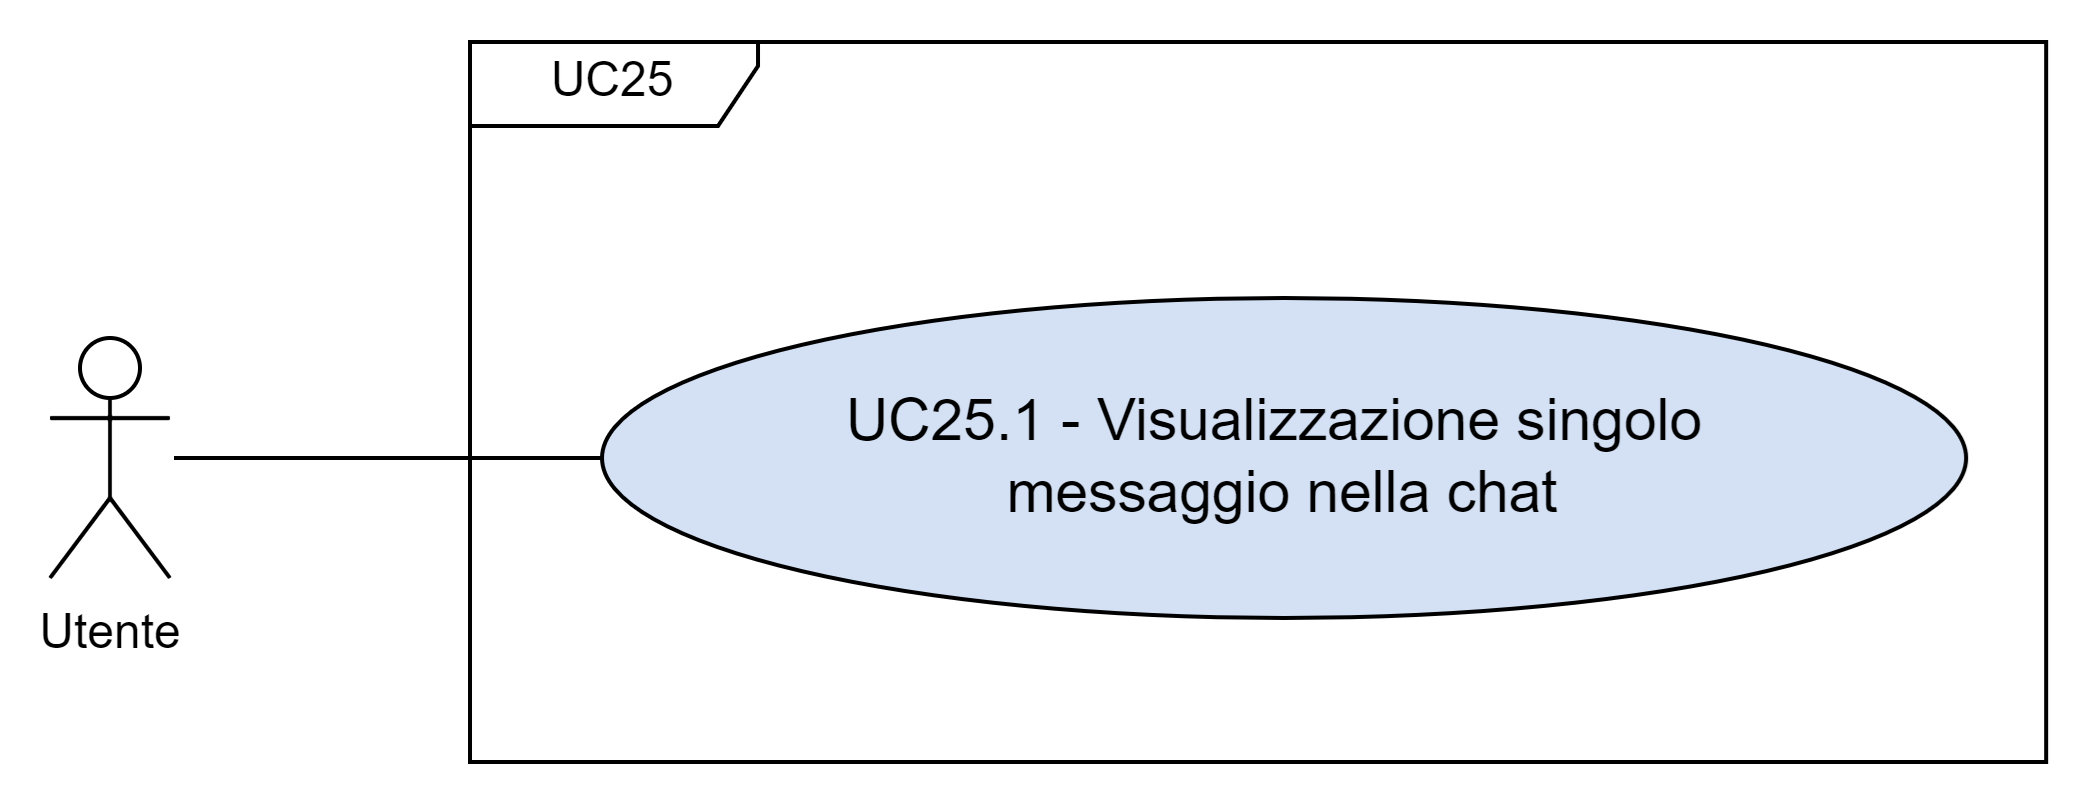
\includegraphics[width=0.90\textwidth]{assets/uc25.png}
  \caption{UC25 - Sottocasi d'uso}
\end{figure}

%%%%%%%%%%%%%%%%%%%%%%%%%%%%%%%%%%%%%%%%%%%%%%%%%%%%%%%%%%%%%%%%%%%%%%%%%%%%%%

\subsubsection{UC25.1 - Visualizzazione singolo messaggio nella chat}\label{UC25point1}
\paragraph*{Descrizione}
L'Utente visualizza un messaggio nella chat.

\paragraph*{Attori principali}
Utente

\paragraph*{Precondizioni}
\begin{itemize}
  \item L'Utente sta visualizzando la lista dei messaggi (\hyperref[UC25]{UC25}).
\end{itemize}

\paragraph*{Postcondizioni}
\begin{itemize}
  \item Il sistema mostra il singolo messaggio nella chat.
\end{itemize}

\paragraph*{Trigger}
L'Utente vuole visualizzare un singolo messaggio all'interno della chat.

\paragraph*{Scenario principale}
\begin{enumerate}
  \item L'Utente visualizza un messaggio.
\end{enumerate}

\paragraph*{Sottocasi d'uso:}
\begin{itemize}
  \item \hyperref[UC25point1point1]{UC25.1.1}: Visualizzazione contenuto messaggio;
  \item \hyperref[UC25point1point2]{UC25.1.2}: Visualizzazione mittente messaggio.
\end{itemize}

\begin{figure}[H]
  \centering
  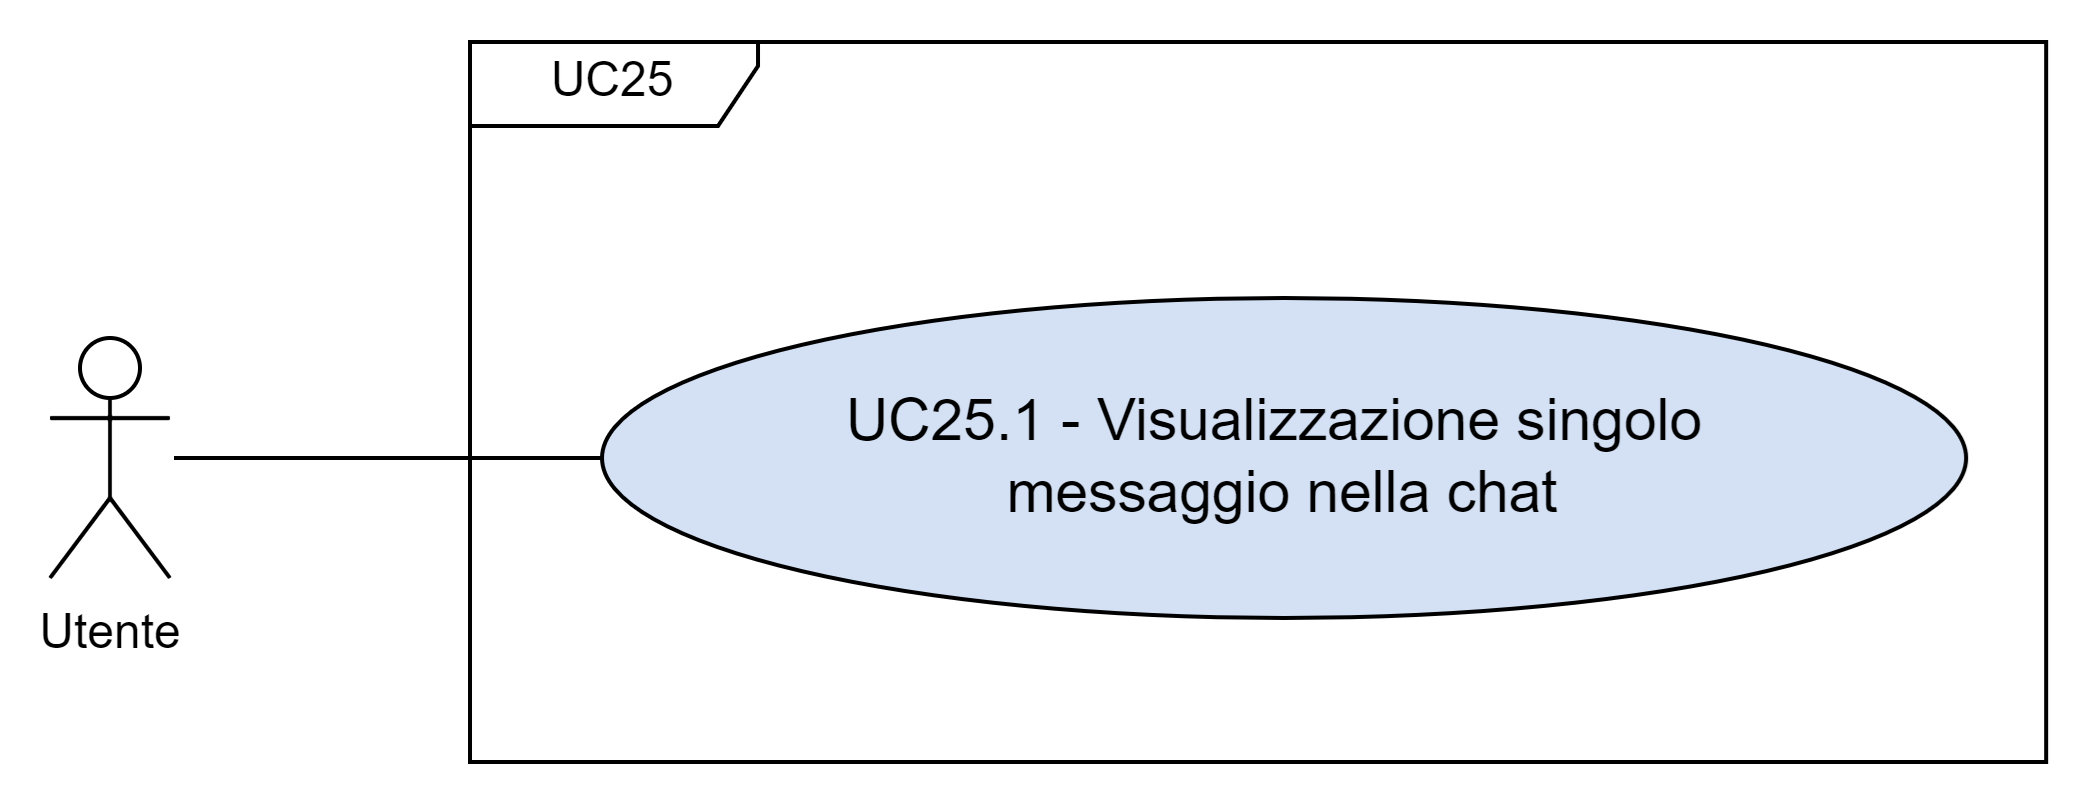
\includegraphics[width=0.90\textwidth]{assets/uc25_1.png}
  \caption{UC25.1 - Sottocasi d'uso}
\end{figure}

%%%%%%%%%%%%%%%%%%%%%%%%%%%%%%%%%%%%%%%%%%%%%%%%%%%%%%%%%%%%%%%%%%%%%%%%%%%%%%

\subsubsection{UC25.1.1 - Visualizzazione contenuto messaggio}\label{UC25point1point1}
\paragraph*{Descrizione}
L'Utente visualizza il contenuto di un messaggio nella chat. 

\paragraph*{Attori principali}
Utente

\paragraph*{Precondizioni}
\begin{itemize}
  \item L'Utente sta visualizzando un singolo messaggio nella chat (\hyperref[UC25point1]{UC25.1}).
\end{itemize}

\paragraph*{Postcondizioni}
\begin{itemize}
  \item Viene visualizzato correttamente il contenuto del messaggio.
\end{itemize}

\paragraph*{Trigger}
L'Utente vuole visualizzare il contenuto di un messaggio all'interno della chat.

\paragraph*{Scenario principale}
\begin{enumerate}
  \item L'Utente visualizza il contenuto di un messaggio.
\end{enumerate}

%%%%%%%%%%%%%%%%%%%%%%%%%%%%%%%%%%%%%%%%%%%%%%%%%%%%%%%%%%%%%%%%%%%%%%%%%%%%%%

\subsubsection{UC25.1.2 - Visualizzazione mittente messaggio}\label{UC25point1point2}
\paragraph*{Descrizione}
L'Utente visualizza il mittente di un messaggio nella chat. Il mittente può essere l'Utente stesso o il ChatBOT.

\paragraph*{Attori principali}
Utente

\paragraph*{Precondizioni}
\begin{itemize}
  \item L'Utente sta visualizzando un singolo messaggio nella chat (\hyperref[UC25point1]{UC25.1}).
\end{itemize}

\paragraph*{Postcondizioni}
\begin{itemize}
  \item Viene visualizzato correttamente il mittente del messaggio.
\end{itemize}

\paragraph*{Trigger}
L'Utente vuole visualizzare il mittente di un messaggio all'interno della chat.

\paragraph*{Scenario principale}
\begin{enumerate}
  \item L'Utente visualizza il mittente di un messaggio.
\end{enumerate}
\subsubsection{UC26 - Selezione DBMS}\label{UC26}

\paragraph*{Descrizione}
L'Utente seleziona un \glossario{DBMS} tra quelli disponibili. La scelta del DBMS è un passaggio chiave nella generazione del prompt. Sebbene \glossario{SQL} sia un linguaggio standard, esistono variazioni specifiche per ogni DBMS. Per garantire che un \glossario{LLM} generi una \glossario{query} SQL corretta, il prompt deve indicare anche il DBMS di destinazione.

\paragraph*{Attori principali}
Utente

\paragraph*{Precondizioni}
\begin{itemize}
  \item L'applicazione è stata avviata con successo;
  \item L'interfaccia per la selezione del \glossario{DBMS} è accessibile.
\end{itemize}

\paragraph*{Postcondizioni}
\begin{itemize}
  \item Il \glossario{DBMS} è stato selezionato correttamente.
\end{itemize}

\paragraph*{Scenario principale}
\begin{enumerate}
  \item L'Utente visualizza la lista dei \glossario{DBMS} disponibili;
  \item L'Utente sceglie un \glossario{DBMS} da una lista predefinita. La scelta è tra i seguenti DBMS:
    \begin{itemize}
      \item MySQL;
      \item MariaDB;
      \item PostgreSQL;
      \item Microsoft SQL Server;
      \item Oracle Database;
      \item SQLite.
    \end{itemize} 
\end{enumerate}
\subsubsection{UC27 - Eliminazione cronologia della chat}\label{UC27}

\begin{figure}[H]
  \centering
  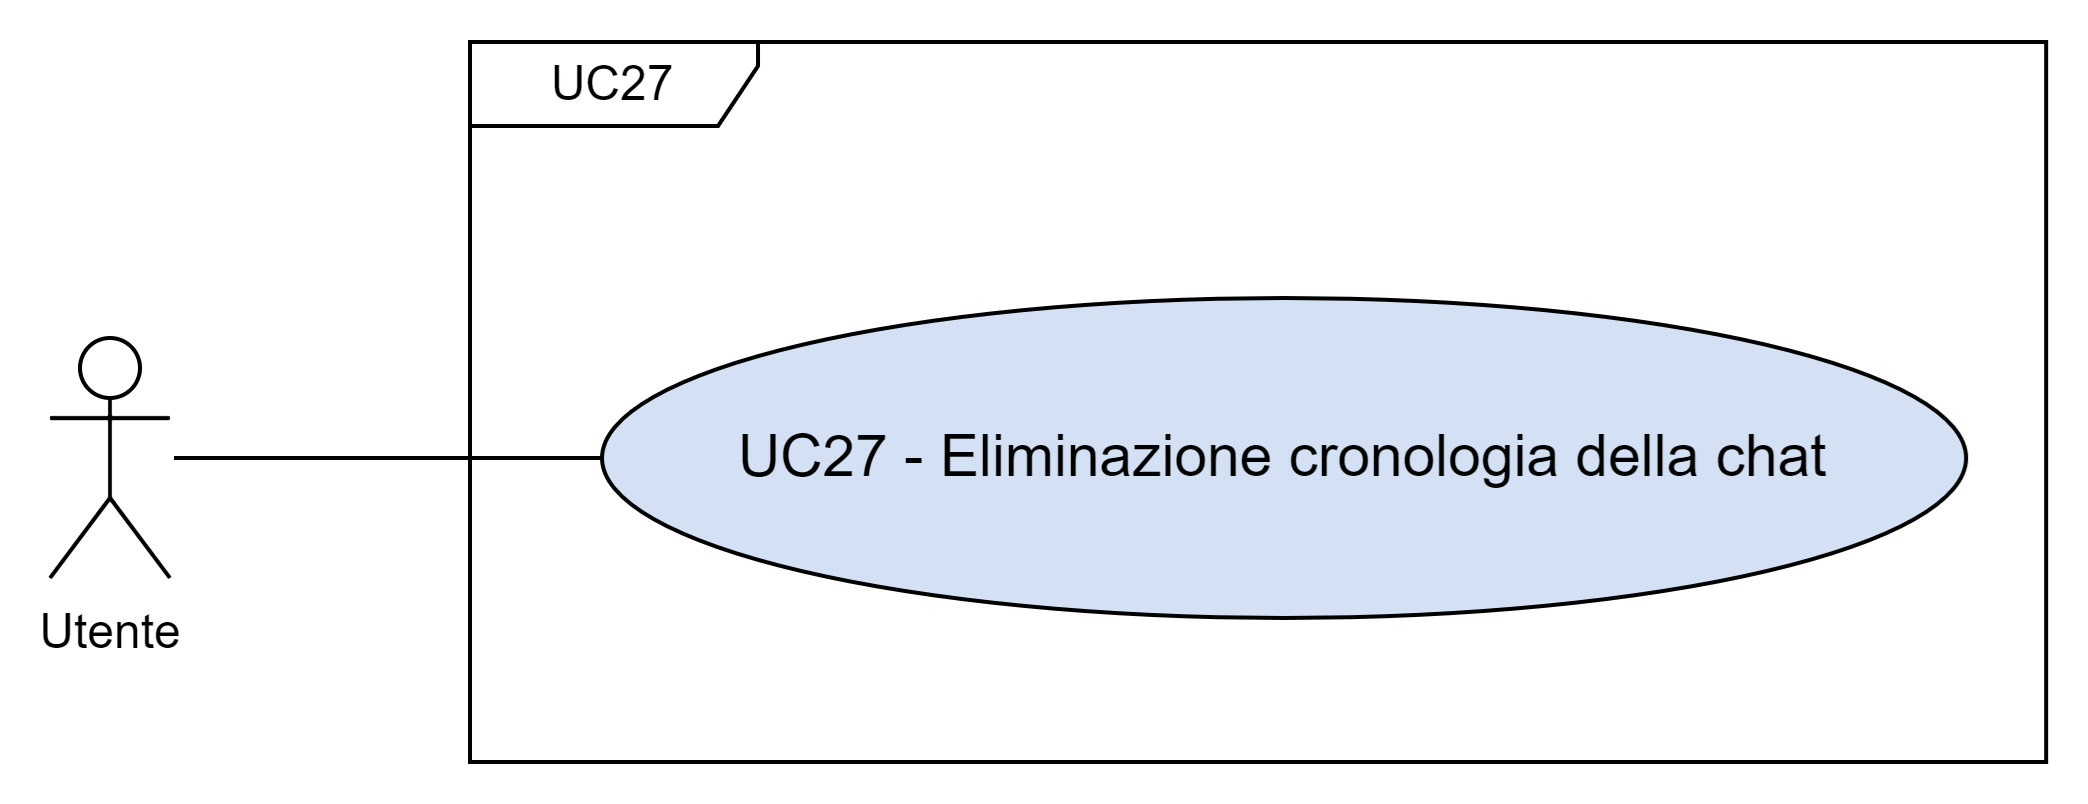
\includegraphics[width=0.90\textwidth]{assets/uc27.png}
  \caption{UC27}
\end{figure}

\paragraph*{Descrizione}
L'Utente elimina la cronologia della chat. La chat è composta da un elenco di messaggi, che possono essere richieste dell'utente o risposte del ChatBOT.

\paragraph*{Attori principali}
Utente

\paragraph*{Precondizioni}
\begin{itemize}
  \item L'applicazione è stata avviata con successo;
  \item È presente almeno un messaggio all'interno della chat.
\end{itemize}

\paragraph*{Postcondizioni}
\begin{itemize}
  \item La cronologia della chat è stata eliminata.
\end{itemize}

\paragraph*{Trigger}
L'Utente vuole eliminare la cronologia della chat.

\paragraph*{Scenario principale}
\begin{enumerate}
  \item L'utente accede alla chat;
  \item L'utente seleziona l'opzione per eliminare la cronologia della chat;
  \item La cronologia della chat viene eliminata.
\end{enumerate}

